\documentclass{report}

% Language setting
% Replace `english' with e.g. `spanish' to change the document language
\usepackage[english]{babel}
\usepackage{blindtext}
\usepackage{titlesec}

% Useful packages
\usepackage{amsmath}
\usepackage{float}
\usepackage{caption}
\usepackage[skip=0.5ex]{subcaption}
\usepackage{graphicx}
\usepackage{xcolor}
\usepackage[
colorlinks=true,urlcolor=blue,linkcolor=purple,citecolor=red
]{hyperref}
\usepackage[toc]{appendix}
\usepackage{markdown}

\usepackage[table,xcdraw]{xcolor}
\usepackage{adjustbox}

% Set page size and margins
% Replace `letterpaper' with `a4paper' for UK/EU standard size
\usepackage[a4paper,top=2cm,bottom=2cm,left=3cm,right=3cm,marginparwidth=1.75cm]{geometry}

% Code listings
\usepackage{listings}
\colorlet{punct}{red!60!black}
\definecolor{background}{HTML}{EEEEEE}
\definecolor{delim}{RGB}{20,105,176}
\colorlet{numb}{magenta!60!black}

\usepackage{listings}
\lstset{basicstyle=\ttfamily}
\lstset{breaklines=true}

\lstdefinelanguage{json}{
	basicstyle=\normalfont\ttfamily,
	numbers=left,
	numberstyle=\scriptsize,
	stepnumber=1,
	numbersep=8pt,
	showstringspaces=false,
	breaklines=true,
	frame=lines,
	backgroundcolor=\color{background},
	literate=
	*{0}{{{\color{numb}0}}}{1}
	{1}{{{\color{numb}1}}}{1}
	{2}{{{\color{numb}2}}}{1}
	{3}{{{\color{numb}3}}}{1}
	{4}{{{\color{numb}4}}}{1}
	{5}{{{\color{numb}5}}}{1}
	{6}{{{\color{numb}6}}}{1}
	{7}{{{\color{numb}7}}}{1}
	{8}{{{\color{numb}8}}}{1}
	{9}{{{\color{numb}9}}}{1}
	{:}{{{\color{punct}{:}}}}{1}
	{,}{{{\color{punct}{,}}}}{1}
	{\{}{{{\color{delim}{\{}}}}{1}
	{\}}{{{\color{delim}{\}}}}}{1}
	{[}{{{\color{delim}{[}}}}{1}
	{]}{{{\color{delim}{]}}}}{1},
	morestring=[b]",
}

\lstdefinelanguage{curl}{
	basicstyle=\normalfont\ttfamily,
	numbers=left,
	numberstyle=\scriptsize,
	stepnumber=1,
	numbersep=8pt,
	showstringspaces=false,
	breaklines=true,
	frame=lines,
	backgroundcolor=\color{background},
	literate=
	*{0}{{{\color{numb}0}}}{1}
	{1}{{{\color{numb}1}}}{1}
	{2}{{{\color{numb}2}}}{1}
	{3}{{{\color{numb}3}}}{1}
	{4}{{{\color{numb}4}}}{1}
	{5}{{{\color{numb}5}}}{1}
	{6}{{{\color{numb}6}}}{1}
	{7}{{{\color{numb}7}}}{1}
	{8}{{{\color{numb}8}}}{1}
	{9}{{{\color{numb}9}}}{1}
	{:}{{{\color{punct}{:}}}}{1}
	{,}{{{\color{punct}{,}}}}{1}
	{\{}{{{\color{delim}{\{}}}}{1}
	{\}}{{{\color{delim}{\}}}}}{1}
	{[}{{{\color{delim}{[}}}}{1}
	{]}{{{\color{delim}{]}}}}{1},
	morestring=[b]",
}


\lstdefinelanguage{ino}{
	basicstyle=\normalfont\ttfamily,
	numbers=left,
	numberstyle=\scriptsize,
	stepnumber=1,
	numbersep=8pt,
	showstringspaces=false,
	breaklines=true,
	frame=lines,
	backgroundcolor=\color{background},
	literate=
	*{0}{{{\color{numb}0}}}{1}
	{1}{{{\color{numb}1}}}{1}
	{2}{{{\color{numb}2}}}{1}
	{3}{{{\color{numb}3}}}{1}
	{4}{{{\color{numb}4}}}{1}
	{5}{{{\color{numb}5}}}{1}
	{6}{{{\color{numb}6}}}{1}
	{7}{{{\color{numb}7}}}{1}
	{8}{{{\color{numb}8}}}{1}
	{9}{{{\color{numb}9}}}{1}
	{:}{{{\color{punct}{:}}}}{1}
	{,}{{{\color{punct}{,}}}}{1}
	{\{}{{{\color{delim}{\{}}}}{1}
	{\}}{{{\color{delim}{\}}}}}{1}
	{[}{{{\color{delim}{[}}}}{1}
	{]}{{{\color{delim}{]}}}}{1},
	morecomment=[l][\color{gray}]{//},
	morestring=[b][\color{violet}]",
	morekeywords={const, void, char, int, float}, keywordstyle=\color{red},
}

\usepackage{csquotes}
\usepackage[
backend=biber,
style=ieee,
]{biblatex}
\addbibresource{sources.bib}

\pagestyle{headings}

\title{Enabling photodetection electronics for 
	fluorescent diamond based quantum sensing}
\author{Vladislav Serafimov}

\begin{document}
	\maketitle
	
	
	
	\tableofcontents
	\chapter{Foreword}
	%This project was done as a graduation thesis for the Ambient Intelligence (AmI) research group at Saxion. I had a pleasant time working on this assignment and collaborating with the members of AmI. The professional environment was very productive and the facilities provided by AmI helped greatly with the project work.
	
	%I would like to thank the people who supported me throughout this project: my internship coach, Eyuel Ayele, and my Saxion coach, Yanin Kasemsinsup. The completion of the assignment is due in no small part to their constant guidance and advice. 
	
	\chapter{Summary}
	% be more specific
	% change question
	% specify stages of the question answering process
	% address 
	
	%An important part of the report is a summary. A summary is used to make clear to other possible interested parties, e.g., 
	%the management, the major purpose / problem / question to be solved / answered, how this has been tackled and the 
	%result of the assignment. 
	%Requirements on a summary:
	%• It must be readable independent from the report, it is not allowed to refer to chapters, figures.
	%• It does not contain figures or tables.
	%• It must summarise:
	%Why the project has been carried out (problem and goal)
	%The used methodology
	%The result (verification with the goal)
	%Major conclusions
	%Major recommendations
	%• It must be written in English, maximum 1 A4
	
	
	\chapter{Abbreviations and terminology}
	\begin{itemize}
		\item{CW - Constant-Wave}
		\item{ECAD - Electronic Computer-Aided Design}
		\item{GUI - Graphical User Interface}
		\item{MRI - Magnetic Resonance Imaging}
		\item{MW - MicroWave}	
		\item{NV - Nitrogen Vacancy}
		\item{ODMR - Optically Detected Magnetic Resonance}
		\item{OLIA - Open Lock-In Amplifier}
		\item{PCB - Printed Circuit Board}
	\end{itemize}
	
	\chapter{Introduction}
This chapter introduces the assignment and some foundational concepts of quantum sensing.

\section{Background}\label{chap:background}
\gls{nv} centers \cite{enwiki:1301369588} are imperfections in the atomic structure of diamonds. The two types of \gls{nv} centers are \gls{nv}0 and \gls{nv}-, as seen in Figure \ref{fig:nvcenter}, but the \gls{nv}- structure is much more commonly used in quantum applications. These imperfections have the useful property of spin-dependent luminescence. This means that the spin of the \gls{nv} center affects the frequency of the light emitted by the structure\footnote{The \gls{nv} center only emits light after absorbing photons, a phenomenon called photoluminescence \cite{enwiki:1309081879}}. Using this quality of the \gls{nv} structure, different environmental metrics (e.g magnetic fields) can be measured. 

The Applied Nanotechnology research group is working on a \gls{nv}-center-based sensor setup. There exist several quantum protocols, but the one this setup needs to support is called \gls{cwodmr}. At its core, \gls{odmr} is a set of protocols, which can detect magnetic fields based on the fluctuations in the fluorescence of \gls{nv} centers \cite{enwiki:1301371272}. \gls{cwodmr} in particular involves exposing the \gls{nv} center to a \gls{mw} sweep while illuminating it with a constant light source. This is in contrast with \gls{podmr} techniques, which use different \gls{ttl} pulse schemes \cite{sewani2020coherent} to modulate the \gls{mw} signal and the light source.

Processing data from the setup requires working with weak signals that are hard to distinguish from the environmental noise. While this is a significant problem, it is also a very common one. Because of this, there is already widely-used system used to isolate signals in such cases: the lock-in amplifier.

\begin{figure}[ht]
	\centering
	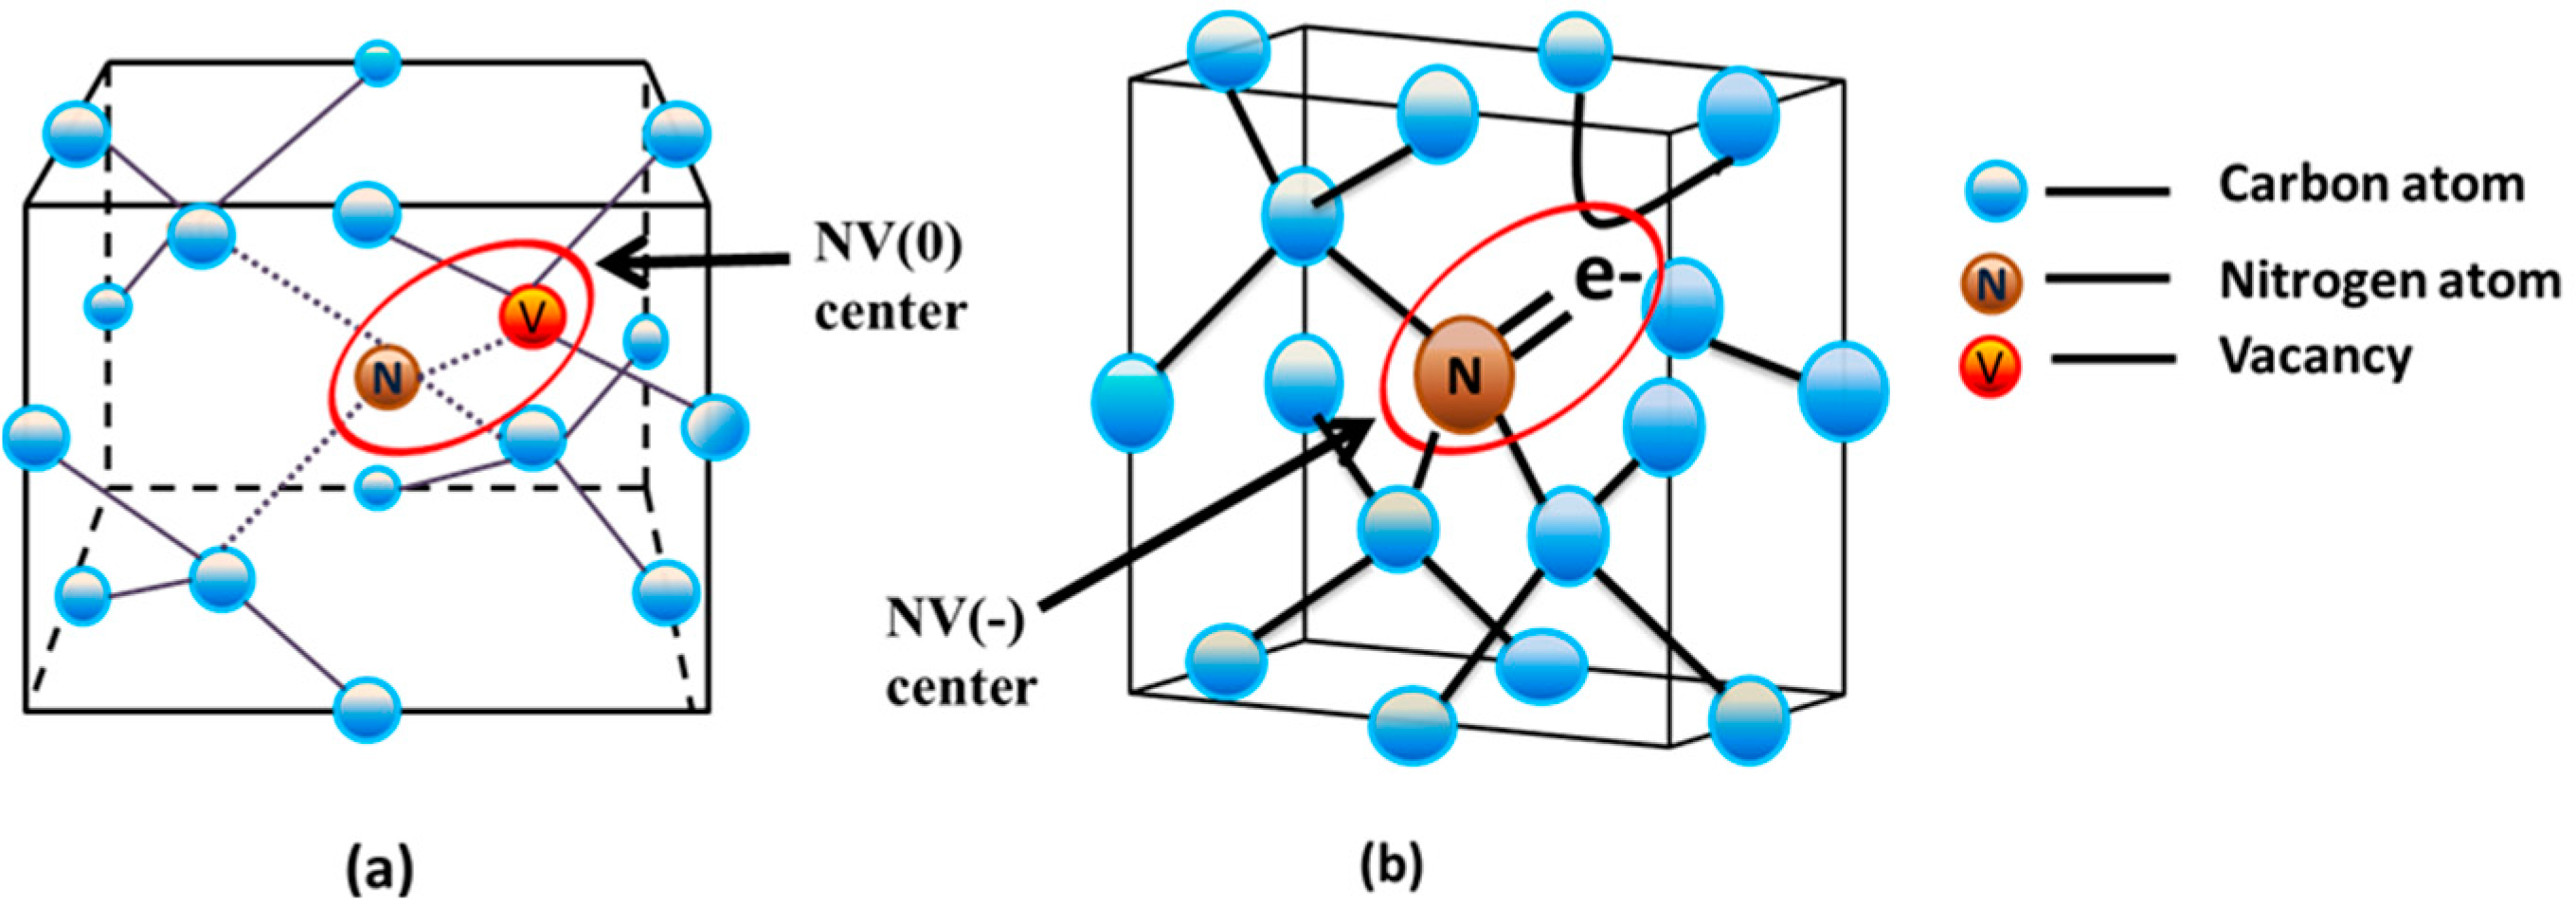
\includegraphics[width=0.7\linewidth]{img/nv_center}
	\caption{\gls{nv}0 (a) and \gls{nv}- (b) structures in diamonds (image credit to Haque et al \cite{haque2017overview})}
	\label{fig:nvcenter}
\end{figure}


\section{Purpose of the assignment}\label{purpose}
Implementing a lock-in amplifier is the main purpose of the assignment. To create a complete solution, there are several different functionalities and systems that need to be developed. 

Before doing anything else, the raw sensor data needs to be extracted and then fed to a lock-in amplifier. This should be done in a standardized manner, in order to facilitate testing with different devices. After establishing connection, a control interface needs to be implemented. It needs to be programmed so that it can control all necessary features of the lock-in amplifier. Following the development of the program, a custom photodetection circuit needs to be designed. The circuit should accommodate the sensors and lock-in amplifier. Lastly, an \gls{olia} \footnote{\gls{olia} is an open-source microcontroller-based lock-in amplifier. It uses common components, which makes it easy to build \cite{harvie2023olia}} circuit needs to be tested and compared to conventional lock-in systems. 


\section{Assignment specifications}\label{specifications}
As already explained, the assignment is quite broad and involves both hardware and software, causing the need for a number of different tools. 

Most of the hardware tools are already available at the Applied Nanotechnology lab. The lock-in amplifiers which will be used for the tests are the most important pieces of hardware. Zurich Instruments HF2LI is the benchmark lock-in amplifier. The target amplification is at least 10dB. There are also several different photodetectors available and the one which fits the project best will be picked at a later date. Chapter \ref{chap:background} already discussed the basics of the \gls{cwodmr} protocol. In order to get an operational \gls{cwodmr} setup, an \gls{mw} generator and a laser will be used. \gls{mw} sweeping needs to be done in the range of 2,8 - 2,9 GHz and the lab already has a custom-built \gls{mw} generator that can output these frequencies. The laser is mostly outside the scope of the assignment, as it is almost entirely optical in nature. Setting it up, together with the \gls{nv} samples, is up to the client. However, it is important to note that the fluorescence wavelength should be in the range of 637 - 800 nm, as it plays an important part in reading the \gls{cwodmr} data.
	
In terms of software, there is more freedom of choice. Interfacing with the HF2LI is done through proprietary software, but this is the only required program. There are various \gls{ecad} software suites that offer the same base functionality. KiCad was selected because the client prefers open-source software. The program for retrieving data from the lock-in amplifiers can be written in both Python and MATLAB. Both languages have good integration with the main lock-in amplifier. They also offer \gls{gui} programming capabilities and are good for scientific computing overall.



\section{Scope of work}
%The scope of the project was extensively discussed with the company coach to ensure the wishes of AmI were feasible and clearly presented. The discussion resulted in the goals presented in this chapter and the MoSCoW prioritization list in Chapter \ref{analaysis_of_specs}

\subsection{Project boundaries}\label{project_boundaries}
% specify what moscow is and put it in front of the goals
The project boundaries were initially based on the assignment form, but were later discussed with the client and refined further. 

\textbf{Must have}
\begin{itemize}
	\item Hardware platform for photodetection
	\item Software for signal processing and visualization
\end{itemize}

\textbf{Should have}
\begin{itemize}
	\item Tests with different diamond samples
\end{itemize}

\textbf{Could have}
\begin{itemize}
	\item Tests with different quantum protocols
	\item \gls{olia} implementation
	\item Tests comparing \gls{olia} to market solutions
\end{itemize}

\textbf{Will not have}
\begin{itemize}
	\item Laser as a part of the hardware platform
	\item Driver upgrade
\end{itemize}


\subsection{Goals} \label{chap:goals}
% goals are tasks now, change to goals
Based on the MoSCoW priorities from Chapter \ref{project_boundaries}, a set of goals was created to further specify all items from each prioritization category. Every goal was designed so that its outcome results in a tangible project milestone (e.g. a deliverable).

\begin{itemize}
	\item[Goal 1]: Create a hardware setup, which measures and amplifies photodiode signals
	\item[Goal 2]: Develop software to process and visualize lock-in amplifier signals
	\item[Goal 3]: Compare the performance of different lock-in amplifiers
\end{itemize}

While these goals are practical, they are still not specific enough. To eliminate the possibility of confusion, a set of tasks were created. All tasks contribute to one of the three goals.

\begin{itemize}
	\item[Task 1.1]: Design a photodiode \gls{pcb}, which can accommodate different lock-in amplifiers
	\item[Task 1.2]: Build an operable \gls{olia}
	\item[Task 2.1]: Develop software that acquires signals and is then able to visualize them
	\item[Task 3.1]: Use key performance metrics to compare the \gls{olia} implementation to market solutions
	\item[Task 3.2]: Measure \gls{olia} performance using different diamond samples and quantum protocols
\end{itemize}

\textbf{Task 1.1} involves the design and production of a photodiode \gls{pcb}. The \gls{pcb} has to output signals that are not only compatible with lock-in amplifiers that are available on the market, but also with the \gls{olia}. This part of the hardware design has the highest priority, which is why it will be done first. 

\textbf{Task 1.2} is to build an \gls{olia} amplifier, which can be used at Applied Nanotechnology's laboratory. This will be done with the technical specifications and firmware provided by Harvie and de Mello \cite{harvie2023olia}. The necessity for an \gls{olia} is low, because the Applied Nanotechnology research group already has two lock-in amplifiers.

\textbf{Task 2.1} is to write an application in Python or MATLAB. This can be done on a different setup, but ideally it will use the hardware setup from \textbf{goal 1}. Because the \gls{olia} project uses open-source firmware that differs from proprietary solutions, there might need to be two separate applications. This task can only be completed once a measurement setup is built, so its execution will follow the first two tasks.

\textbf{Task 3.1} requires all previous tasks to be finished. The completed setup needs to be used to measure the performance of lock-in amplifiers available on the market and the \gls{olia} implementation. SNR, bandwidth and stability are the main metrics that need to be compared.

\textbf{Task 3.2} is similar to \textbf{task 3.1}, but it is a much broader exploration of the performance of the lock-in amplifiers. Using different diamond samples and quantum protocols will show how the amplifier performs and how different conditions affect it. Because the task can be used to verify the setup from \textbf{goal 1}, it can also be done before \textbf{task 3.1}. Tests with varying diamond samples are more important to the client, which is why they will take precedence over tests with different quantum protocols.


\subsection{Deliverables}
The description of the tasks already provided context for the deliverables, but this subsection contains a formalized version of the deliverables.

\begin{enumerate}
	\item Photodetection \gls{pcb} 
	\item \gls{olia} implementation
	\item Software application
	\item Comparison visualization
	\item Technical documentation
\end{enumerate}

The only deliverable, which was not mentioned in Chapter \ref{chap:goals} is the technical documentation. This is because it should contain information about every task.

\section{Methodology}\label{methodological_approach}
The V-Model methodology was selected, as it is well-suited for low-level projects. Figure \ref{fig:vmodel} shows a diagram of the phases of the V-Model. Unlike some software-oriented models, the V-Model is very sequential. This can sometimes be seen as detrimental, but in this case it helps with structuring the project. Another benefit of this model is that there are multiple testing activities, which underpin the quality assurance. A contentious feature of the V-Model is the heavy reliance on the initial requirements. This need for deliberate project requirements can be hard to meet, especially if the client representative is not technically proficient. However, this is not the case in this project. The requirements were extensively discussed with the client representative, based on which the project boundaries in Chapter \ref{project_boundaries} were set up.

\begin{figure}[ht]
	\centering
	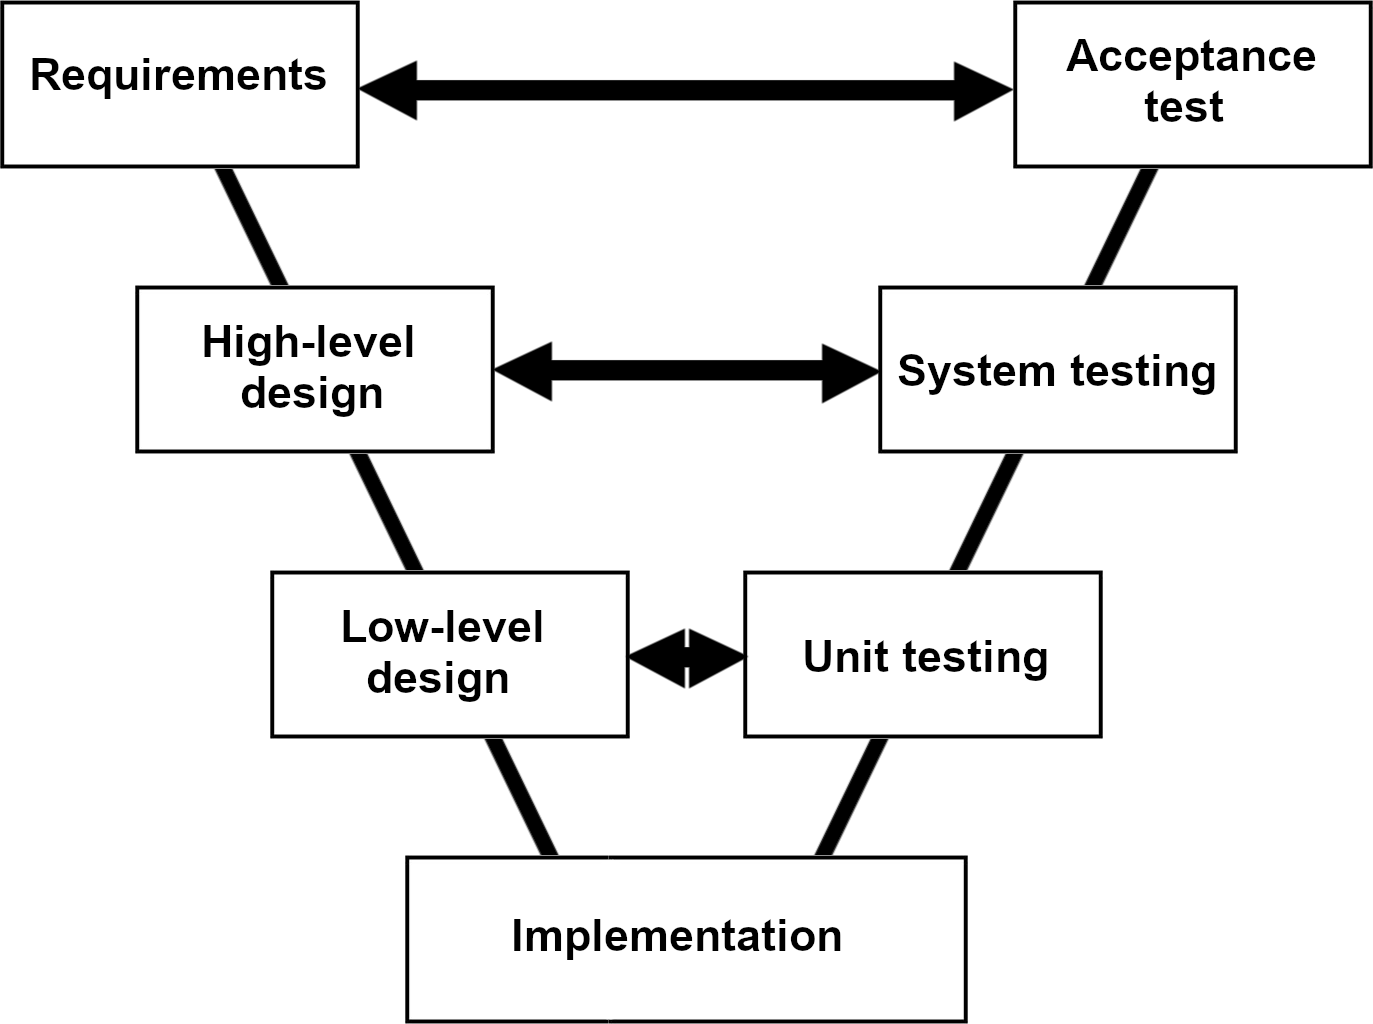
\includegraphics[width=0.7\linewidth]{img/vmodel}
	\caption{V-Model diagram}
	\label{fig:vmodel}
\end{figure}


\section{Report outline}
%TODO: add after everything else is done
%After the introduction, the report can be split into three parts, each corresponding to one of the phases in the waterfall model from Figure \ref{fig:phases}. 

%The functional design chapter introduces all the necessary prerequisite knowledge, which has been explored during the familiarization and research. It also describes the design process as the project moved from research to implementation. 

%After that, the technical design discusses the most important implementation and integration details. It also discusses practical details that might be useful for future work.

%The last three chapters, testing results, conclusion and recommendations, show the outcomes of the tests and present the explanation of those results. They also contain advice for future work, motivated by the test data interpretation and the conclusions drawn from them.

%The appendices are not integral to the report, but might prove useful to people looking to expand on the project.
	

	\chapter{Functional design} \label{chap:func_design}
\section{Background knowledge}
\subsection{Spin states}
Spin, at least in quantum mechanics, is the intrinsic angular momentum of a particle, which is described by the quantum number of the particle. Importantly, it differs from the angular momentum in classical mechanics, which is extrinsic. Spin characterizes systems of particles, usually electrons, using quantum entanglement. This phenomenon refers to the "entanglement", or spin correlation, of a set of particles.

These foundational concepts make it possible to describe quantum systems using various states. The most simple states, used as descriptors, are the energy states. Ground states refer to the system being in an energy minimum. On the other hand, excited states signify that the system has more energy than at its ground state. Additionally, there can be intermediate states during state transition.

While the aforementioned states describe system energy, they have no bearing on the spin. For the purposes of this project, only two spin states need to be explained. The first one is called singlet state. It occurs when an entangled system has a total spin of 0, caused by the mutual cancellation of spin. For example, for a system of two entangled electrons to be a singlet, the two spins would need to point in opposite directions. The second spin state is called triplet and it has a total spin of 1. Triplets can consist of, for instance, two unpaired electrons with aligned spins that sum up to 1. Singlets and triplets both have major distinguishing features and properties, which is why they can be used for quantum sensing. Aside from the difference in spin, triplets tend to have higher energy levels. They also exhibit attraction to magnetic fields, while singlets cannot be influenced directly by magnetism.

%\subsection{Energy levels and state transitions} and Zero-field splitting
\subsection{Zeeman effect}
Discovered by Pieter Zeeman in 1896, the Zeeman effect is another important phenomenon that enables quantum sensing. If under normal circumstances a light-emitting quantum system only emits one spectral line, then when a magnetic field is applied to it the line will split, thus exhibiting the Zeeman effect. In an \gls{nv} center, this phenomenon causes the $\ket{\pm1}$ energy level to split into $\ket{+1}$ and $\ket{-1}$. 

\subsection{Energy levels}\label{chap:energy_levels}
Figure \ref{fig:energylevels} shows the energy level diagram of an \gls{nv} center.

\begin{figure}[ht]
	\centering
	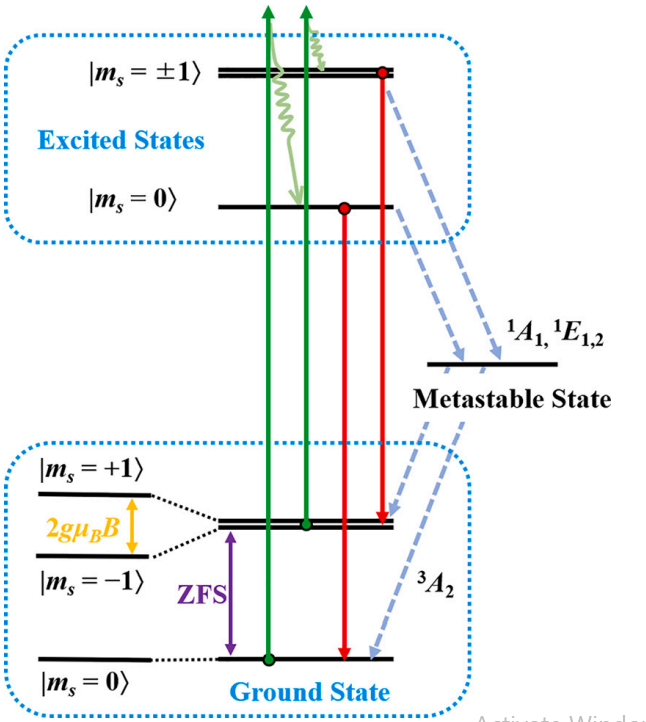
\includegraphics[width=0.7\linewidth]{img/energy_levels}
	\caption{\gls{nv} center energy level diagram (image credit to Song et al \cite{song2024enhancing})}
	\label{fig:energylevels}
\end{figure}

After illuminating the \gls{nv} center with a green laser, electrons go from a ground state to an excited state. They then need to return to the ground state. This decay process is usually direct and emits a red photon, however it can also go through the metastable singlet state and emit an infrared photon. It should be noted that whenever the \gls{nv} center is exposed to the resonant frequency $\nu = 2,87 GHz$ the probability of emitting an infrared photon is significantly increased.


\section{Quantum protocols}
There are a number of different quantum protocols, which differ in what they can measure, in how precisely they can measure it and in the complexity of the hardware they require to operate. \gls{cwodmr} is the main protocol this project is aimed at facilitating. As Saijo et al \cite{saijo2018ac} demonstrate, \gls{cwodmr} is relatively simple, while still detecting magnetic field with reasonable sensitivity. \gls{podmr} does outperform \gls{cwodmr} \cite{zhang2020high}, but because of the added complexity working with it is a "Could have" (see Chapter \ref{project_boundaries}). Before being able to run \gls{podmr} on the setup at the lab, several protocols need to be implemented first \cite{sewani2020coherent}. $T_1$ measurements, which are one of the fundamentals of \gls{mri}, should be conducted first. Afterwards, Rabi oscillations need to be observed and measured in order to calibrate the setup. Without these intermediate protocols, \gls{podmr} cannot be performed.



\subsection{\glsfmtshort{cwodmr}}
\gls{cwodmr} is a quantum protocol that has seen extensive usage in sensing setups that measure magnetic fields. Its working principle is centered around the photoluminescence of \gls{nv} centers and the difference in light emission based on spin states. As already discussed in Chapter \ref{chap:energy_levels}, the \gls{nv} center emits less visible light when at the resonant frequency $\nu$. Additionally, two more dips appear on the spectrum if a magnetic field is applied.Calculating the magnetic field can be done using the formula $h\nu = g_e\mu_BB_{AC}$ \footcite[In the formula, $h$ is the Planck constant, $g_e$ is the g-factor of the electron and $\mu_B$ is the Bohr magneton. Knowing all other variables, $B_{AC}$ can easily be calculated.]{enwiki:1301371272}. Figure \ref{fig:cwodmr} shows an example of what a \gls{cwodmr} spectrum might look like. 

\begin{figure}[ht]
	\centering
	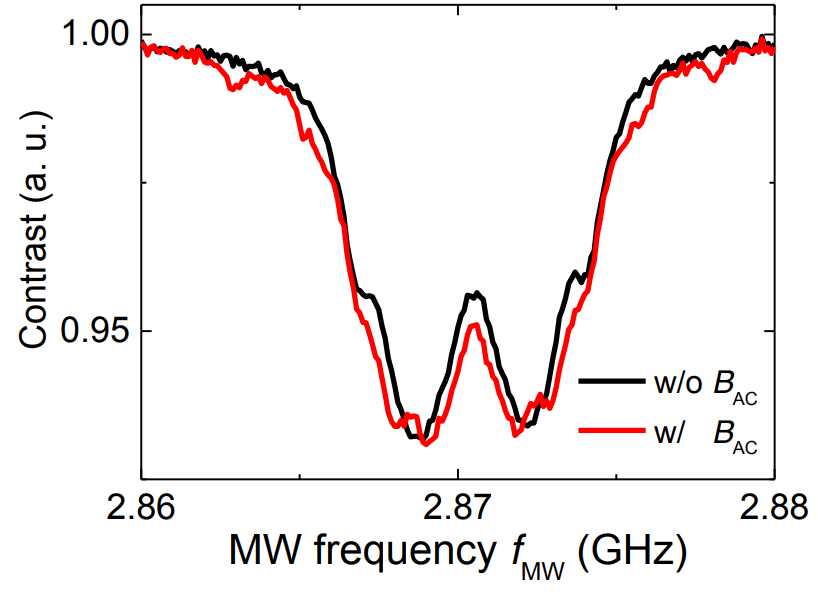
\includegraphics[width=0.7\linewidth]{img/cw_odmr}
	\caption{Example of a \gls{cwodmr} spectrum \textbf{\textcolor{red}{with}} and \textbf{without} a magnetic field (image credit Saijo et al \cite{saijo2018ac})}
	\label{fig:cwodmr}
\end{figure}


\subsection{$T_1$ relaxometry}
$T_1$, $T_2$ and $T_2^*$ relaxation time measurements are commonly associated with radiometry \cite{ballinger23}, but they have other uses too. $T_1$ measurements, in particular, are useful in the realm of quantum sensing. Knowing the $T_1$ relaxation time, which refers to the time it takes for the spins in an \gls{nv} system to decay back to their original state, makes it possible to adjust the pulse sequences of more complex protocols and thus get better results.  %explain what relaxation is and the protcol

% % alternative to tikz diagram
%\begin{figure}[ht]
%	\centering
%	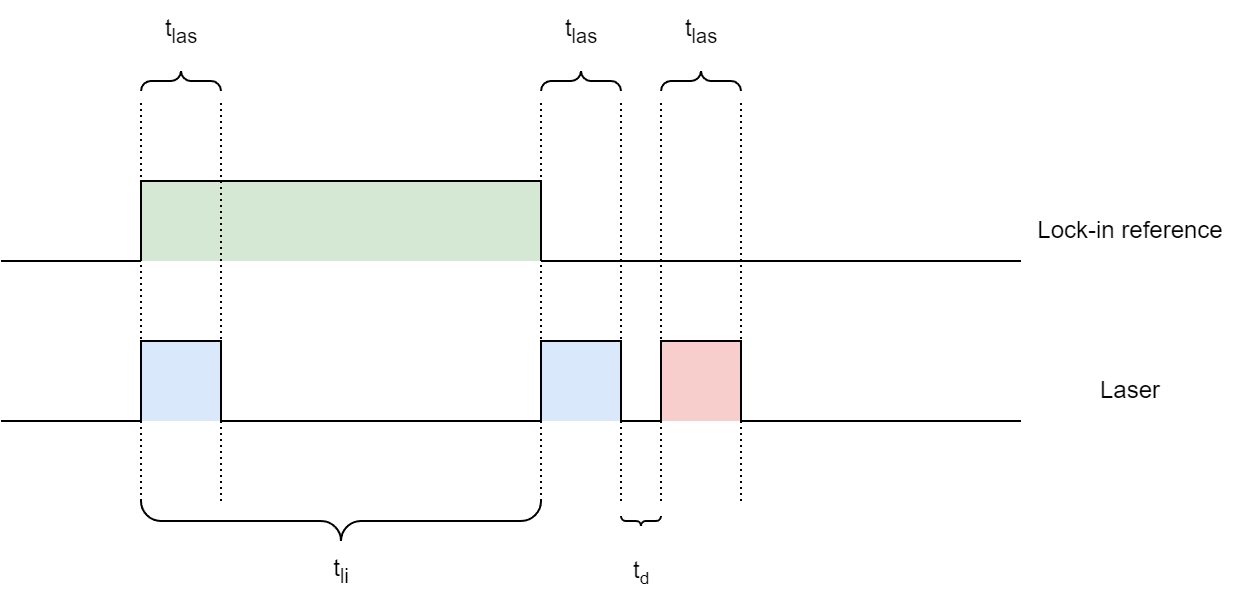
\includegraphics[width=0.9\linewidth]{drawio_diagrams/t1_waveforms.drawio}
%	\caption{Laser and reference signals for $T_1$ measurements}
%	\label{fig:t1waveforms}
%\end{figure}

\begin{figure}[ht]
	\centering
	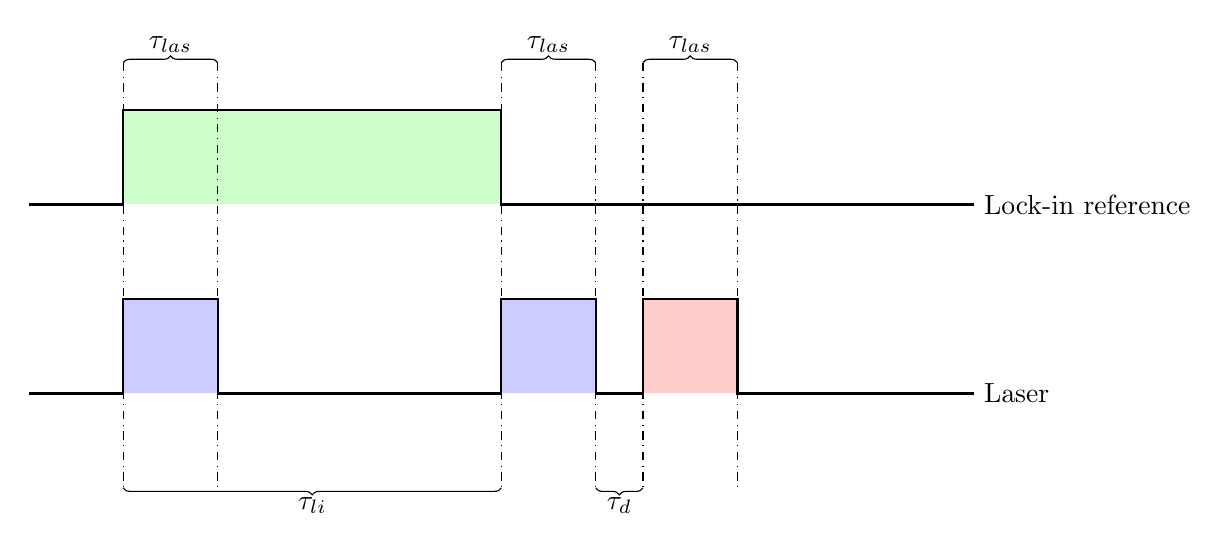
\begin{tikzpicture}[scale=.3]
		% TTL signal rectangles
		\fill [blue!20] 		(4,0) 	rectangle (8,4);
		\fill [blue!20] 		(20,0) 	rectangle (24,4);
		\fill [red!20]			(26,0)	rectangle (30,4);
		\fill [green!20] 		(4,8) 	rectangle (20,12);
		
		% signal lines
		\draw [thick] (0,0) -- (4, 0) -- (4,4) --(8,4) -- (8,0) -- (20,0) -- (20,4) -- (24,4) --(24,0) -- (26,0) -- (26,4) -- (30,4) -- (30,0) -- (40,0) node[anchor=west]{Laser};
		\draw [thick] (0,8) -- (4,8) -- (4,12) -- (20,12) -- (20,8) -- (40,8) node[anchor=west]{Lock-in reference}; % ref
		
		% curly braces top
		\draw [decorate, decoration={brace}] (4,14) -- (8,14) node[midway, above]{$\tau_{las}$};
		\draw [decorate, decoration={brace}] (20,14) -- (24,14) node[midway, above]{$\tau_{las}$};
		\draw [decorate, decoration={brace}] (26,14) -- (30,14) node[midway, above]{$\tau_{las}$};
		
		% curly braces bottom
		\draw [decorate, decoration={brace, mirror}] (4,-4) -- (20,-4) node[midway, below]{$\tau_{li}$};
		\draw [decorate, decoration={brace, mirror}] (24,-4) -- (26,-4) node[midway, below]{$\tau_{d}$};
		
		% dash-dotted lines
		\draw [dash dot] (4,14) -- (4,-4);
		\draw [dash dot] (8,14) -- (8,-4);
		\draw [dash dot] (20,14) -- (20,-4);
		\draw [dash dot] (24,14) -- (24,-4);
		\draw [dash dot] (26,14) -- (26,-4);
		\draw [dash dot] (30,14) -- (30,-4);
		
	\end{tikzpicture}
	\caption{Laser and reference signals for $T_1$ measurements}
	\label{fig:t1waveforms}
\end{figure}





The waveforms which are needed for $T_1$ measurements are shown if Figure \ref{fig:t1waveforms}. While both are important in practice, the lock-in is not as relevant, at least in this section of the report. However, its working principle is explored in Chapter \ref{chap:lockin}. For now, all that needs to be said about the lock-in reference signal is that it is periodic and $\tau_{li}$ is much longer than $\tau_{las}$ (Sewani et al \cite{sewani2020coherent} propose $\tau_{li} = 15 ms$ and $\tau_{las} = 5 \mu s$). Laser pulses, on the other hand, are not periodic. Instead, there are three short pulses every reference period (which is $2\tau_{li} s$ long). The two blue pulses have the same timing every cycle, because they initialize the \gls{nv} spins. However, the red pulse always occurs after the variable dark time $\tau_d$. Depending on the $T_1$ decay at the time of the readout pulse, a different voltage will be detected. Figure \ref{fig:t1result} shows what results can be expected when measuring $T_1$. Determining the value of $T_1$ is done using Formula \ref{eq:t1}, where $I$ is the light intensity, $I_\infty$ is the light intensity offset and $\tau_d$ is the dark time. 

\begin{equation}\label{eq:t1}
I(t)=I_\infty+I(0)e^{-\tau_d/T_1}
\end{equation}



\begin{figure}[ht]
	\centering
	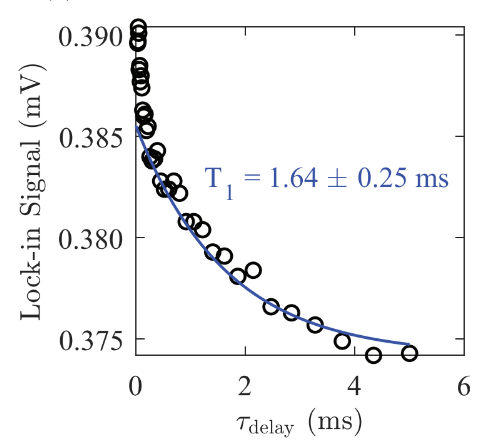
\includegraphics[width=0.7\linewidth]{img/t1_result}
	\caption{Results of a set of $T_1$ measurements with varied dark time $\tau_d$ (image credit to Sewani et al \cite{sewani2020coherent})}
	\label{fig:t1result}
\end{figure}



\subsection{\glsfmtshort{podmr}}
As a descriptor \gls{podmr} is somewhat vague, which is why it has been used for a number of protocols. Different pulse schemes can result in radically different . Some researches use 

\section{Quantum sensing setup}\label{chap:td:quantum_setup}
Executing all of the aforementioned protocols requires a sensing setup with some specific capabilities. This section discusses the devices that make up the setup and the functionalities require by each protocol.

A high-level diagram of the quantum sensing system can be seen in Figure \ref{fig:overview_high_lvl}. There are 2 input devices in the system, but most protocols exclusively use the function generator. On the other hand, only a single lock-in amplifier is used as an output device for all measurements. 

The blue boxes show the components responsible for sending and receiving light signals. They constitute the core of the setup. Waveforms are generated by the function generator, no matter the protocol. Using a current driver, the laser is then used to illuminate the diamond sample. The resulting luminescence is then measured by the photodetector and processed by the lock-in amplifier. All protocols need this part of the setup, however they utilize it differently.

Microwave generation, when needed, starts with a \gls{ttl} signal from the function generator or a frequency sweep using a dedicated device. Out of all protocols, only \gls{cwodmr} requires a sweep. The antenna then broadcasts the signal, while the switch isolates the signal generator from it. 

\begin{figure}[ht]
	\centering
	\begin{tikzpicture}[
		% define box styles
		boxr/.style={rectangle, thick, draw=red!50!black, fill=red!5, minimum size=5mm},
		boxg/.style={rectangle, thick, draw=green!50!black, fill=green!5, minimum size=5mm},
		boxb/.style={rectangle, thick, draw=blue!50!black, fill=blue!5, minimum size=5mm},
		]
		% draw MW nodes
		\node[boxg] (fgen)							{Function generator};
		\node[boxr] (mwsw)		[right=10 mm of fgen] 		{\glsfmtshort{mw} switch};
		\node[boxr] (mwant)		[right=of mwsw]		{\glsfmtshort{mw} antenna};
		\node[boxg] (mwsweep)	[above=of mwsw] 	{Frequency sweeper};
		% draw main system nodes
		\node[boxg] (lockin)	[right=of mwant]	{Lock-in amplifier};
		\node[boxb] (driver) 	[below=of fgen]		{Current driver};
		\node[boxb] (laser) 	[below=of mwsw]		{Laser};
		\node[boxb] (nv) 		[below=of mwant] 	{NV sample};
		\node[boxb] (detect) 	[below=of lockin]	{Photodetector};
		

		% draw MW lines
		\draw[->, thick] 			(fgen.east) 		to node[midway, above]{\glsfmtshort{ttl}} 	(mwsw.west);
		\draw[->, thick] 			(mwsw.east) 		to node[midway, above]{\glsfmtshort{ttl}} 	(mwant.west);
		\draw[->, thick, dashed]	(mwsweep.south) 	to node[midway, left]{Sweep} 				(mwsw.north);
		% draw main system lines
		\draw[->, thick]			(fgen.south)		to node[midway, left]{\glsfmtshort{ttl}} 	(driver.north);
		\draw[->, thick] 			(driver.east) 		to node[midway, above]{Current} 			(laser.west);
		\draw[->, thick]			(laser.east) 		to node[midway, above]{Light} 				(nv.west);
		\draw[->, thick]			(nv.east) 			to node[midway, above]{Light}				(detect.west);		
		\draw[->, thick]			(detect.north) 		to node[midway, right]{Signal}				(lockin.south);	
		% draw long line
		\draw[->, thick] (fgen.south east) .. controls +(down:5mm) .. node[pos=.9, sloped, below]{Reference signal}(lockin.south west);
	\end{tikzpicture}
	\caption{High-level overview of the quantum sensing setup}
	\label{fig:overview_high_lvl}
\end{figure}

\section{Lock-in amplification} \label{chap:lockin}
As a means of retrieving data, lock-in amplification is the most suitable for the setup due to its relatively low cost, signal retrieval capabilities and the possibility of using one amplifier for several setups. 

\begin{figure}[ht]
	\centering
	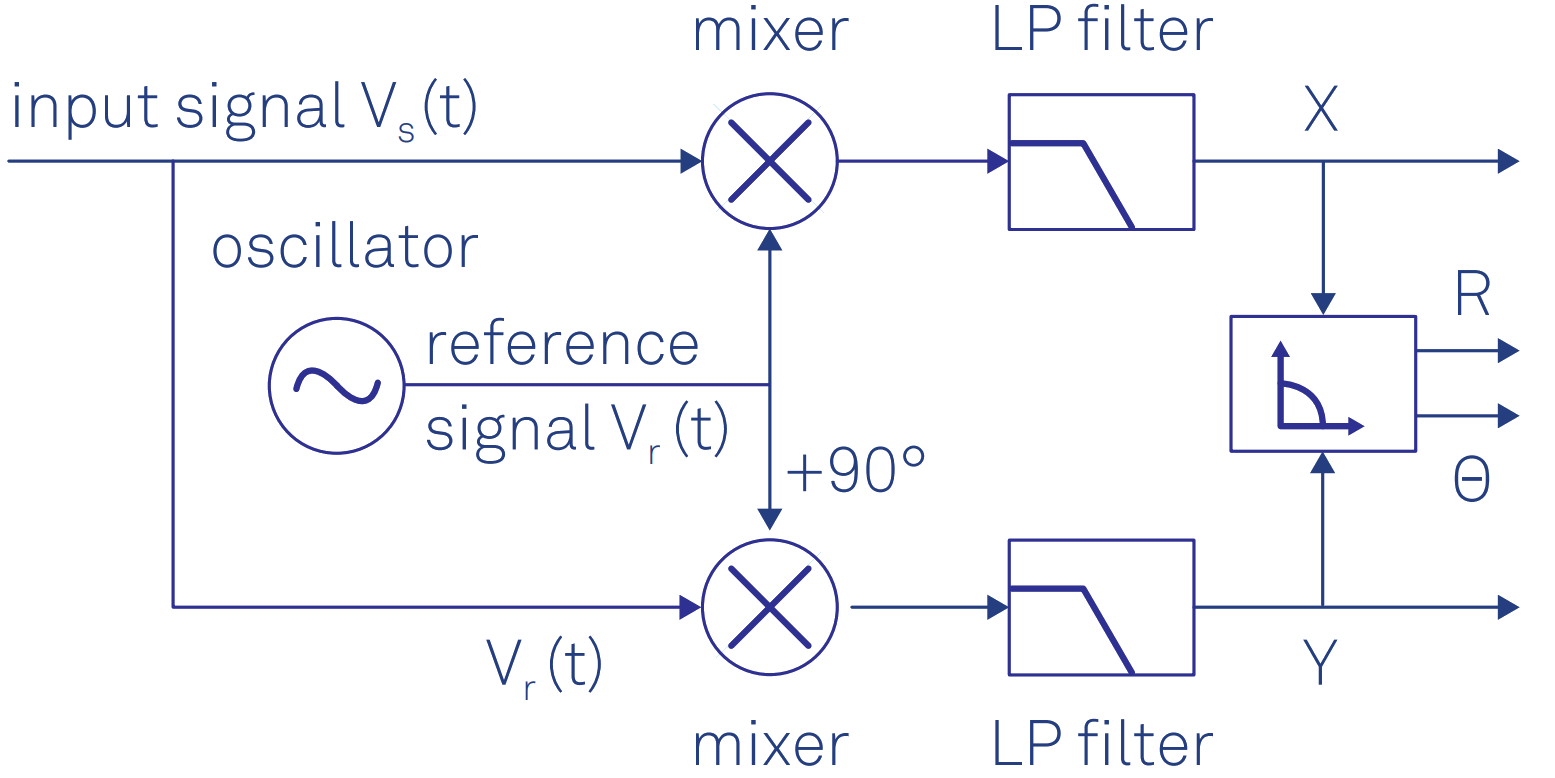
\includegraphics[width=0.7\linewidth]{img/lia_hl_schematic}
	\caption{High-level diagram of a lock-in amplifier (image credit to Zurich Instruments \cite{instruments2018principles})}
	\label{fig:liahlschematic}
\end{figure}

Figure \ref{fig:liahlschematic} shows an overview of how lock-in amplification works. Simply put, the amplifier receives a signal $V_s$ and extracts the data at the frequency of a reference signal $V_r$. To explain this more thoroughly, lock-in amplification utilizes the fact that every signal is made of periodic waves, which are equal to zero when averaged. 

\begin{equation}\label{eq:voltage_sig}
	V_s = R\cos{(\omega_st + \theta)} = \frac{R}{2}e^{i(\omega_st + \theta)} + \frac{R}{2}e^{-i(\omega_st + \theta)}
\end{equation}

Figure \ref{eq:voltage_sig} shows how a simple sine wave signal looks like, where $\omega_s$ is the frequency and $\theta$ is the phase of the signal.

\begin{equation}\label{eq:voltage_ref}
	V_r = e^{-i\omega_rt}
\end{equation}

\begin{equation}\label{eq:voltage_mult}
	V_m = V_sV_r = \frac{R}{2}e^{i(\omega_s -\omega_r)t  + \theta} + \frac{R}{2}e^{-i(\omega_s +\omega_r)t + \theta}
\end{equation}

% Thorlabs Photodiodes and Photoconductors Tutorial:
% https://www.thorlabs.com/newgrouppage9.cfm?objectgroup_id=9020
\section{Photodetection}
Photodetection is how the \gls{nv} photoluminescence is measured, effectively turning light into current using a photodiode. However, a bare photodiode cannot be connected to a lock-in amplifier, because it functions as a current generator. This is where the photodetection \gls {pcb} comes in. Its purpose is to transform the current into voltage and then amplify the resulting signal to the necessary voltage level. 

\subsection{Design process} \label{chap:photodetection_design}
Designing the photodetector is mostly about creating a \gls{tia}, which is a tool used for converting current to voltage, and specifically tuning its parameters so that it works with the selected photodiode under operating conditions. 

\begin{figure}[ht]
	\centering
	\resizebox{.5\textwidth}{!}{%
		\begin{circuitikz}
			\tikzstyle{every node}=[font=\normalsize]
			\draw [ line width=0.5pt](3.75,10.75) to[empty photodiode,l={ \normalsize $D_1$}] (3.75,9);
			\draw [ line width=0.5pt](6.5,10.25) node[op amp,scale=1] (opamp2) {};
			\draw [ line width=0.5pt](opamp2.+) to[short] (5,9.75);
			\draw [ line width=0.5pt] (opamp2.-) to[short] (5,10.75);
			\draw [ line width=0.5pt](7.7,10.25) to[short](8,10.25);
			\draw [line width=0.5pt](5,9) to (5,8.25) node[ground]{};
			\draw [ line width=0.5pt](5,8.5) to[short] (5,9.75);
			\draw [ line width=0.5pt](3.75,10.5) to[short] (3.75,10.75);
			\draw [ line width=0.5pt](3.75,10.75) to[short] (5,10.75);
			\node at (4.5,10.75) [circ] {};
			\draw [ line width=0.5pt](4.5,10.75) to[short] (4.5,13.5);
			\draw [ line width=0.5pt](4.5,12.25) to[short] (5,12.25);
			\draw [ line width=0.5pt](4.5,13.5) to[short] (5,13.5);
			\draw [ line width=0.5pt](7.5,10.25) to[short] (7.5,11);
			\draw [ line width=0.5pt](5,12.25) to[european resistor,l={ \normalsize $R_1$}] (7,12.25);
			\node at (4.5,12.25) [circ] {};
			\draw [ line width=0.5pt](7,12.25) to[short] (7.5,12.25);
			\draw [ line width=0.5pt](7.5,12.25) to[short] (7.5,11);
			\draw [ line width=0.5pt](7.5,12.25) to[short] (7.5,13.5);
			\draw [line width=0.5pt](5,13.5) to[C,l={ \normalsize $C_1$}] (7,13.5);
			\node at (7.5,12.25) [circ] {};
			\draw [ line width=0.5pt](7,13.5) to[short] (7.5,13.5);
			\draw [ line width=0.5pt](8,10.25) to[short, -o] (8.25,10.25) node {$\ \ \ \ \ \ \ \ \ V_{out}$};
			\draw [ line width=0.5pt](3.75,10.75) to[short] (3.75,10.5);
			\draw [line width=0.5pt](3.75,9) to (3.75,8.25) node[ground]{};
			\draw [line width=0.5pt, ->, >=Stealth] (3.25,10.25) -- (3.25,9.25);
			\node [font=\normalsize] at (3,9.75) {$I_f$};
		\end{circuitikz}
	}%
	\caption{Basic \gls{tia} circuit}
	\label{fig:tia}
\end{figure}

The basic circuit, shown in Figure \ref{fig:tia}, is all that is required for photodetection. Following the guidelines for making a \gls{tia} set by Texas Instruments \cite{semig24}, all the parameters of the circuit can be calculated.

\begin{equation}\label{eq:r1}
	R_1 = \frac{V_{o\ max}}{I_{o\ max}}\ \text{assuming}\ V_{o\ min} = 0 \unit{\volt}
\end{equation}

The resistor $R_1$ determines the transimpedance gain of the amplifier. Equation \ref{eq:r1} shows how its value can be calculated by using the output voltage and input current. It should be noted that the minimum output voltage cannot be different from 0 in this use case.

\begin{equation}\label{eq:c1}
	C_1 = \frac{1}{2 \pi R_1 f_{rc}}
\end{equation}

The capacitance of $C_1$ can be calculated using the resistance of $R_1$ and the cutoff frequency $f_{rc}$, as shown in Equation \ref{eq:c1}. 

\begin{equation}\label{eq:gbw}
	f_{c} = (1 + \frac{C_d + C_{cm}}{C_1})f_{rc} \approx f_{rc}
\end{equation}

Even though $f_{rc}$ provides an approximation for the cutoff frequency, the parasitic capacitances in the system will cause it to be slightly bigger. Equation \ref{eq:gbw} shows how a more accurate cutoff frequency $f_c$ can be calculated by taking into account $C_d$ and $C_{cm}$ (differential and common-mode capacitance respectively). In this case, $f_c$ tells us the gain bandwidth or the frequency range in which DC gain is retained.

In addition, a non-inverting amplifier can be added, to increase the gain of the circuit even more, without affecting the phase. Figure \ref{fig:tia_nia} shows how it can be connected to the output of the \gls{tia} from Figure \ref{fig:tia}.

\begin{figure}[!ht]
	\centering
	\resizebox{.9\textwidth}{!}{%
		\begin{circuitikz}
			\tikzstyle{every node}=[font=\normalsize]
			\draw [ line width=0.5pt](3.75,10.75) to[empty photodiode,l={ \normalsize $D_1$}] (3.75,9);
			\draw [ line width=0.5pt](6.5,10.25) node[op amp,scale=1] (opamp2) {};
			\draw [ line width=0.5pt](opamp2.+) to[short] (5,9.75);
			\draw [ line width=0.5pt] (opamp2.-) to[short] (5,10.75);
			\draw [ line width=0.5pt](7.7,10.25) to[short](8,10.25);
			\draw [line width=0.5pt](5,9) to (5,8.25) node[ground]{};
			\draw [ line width=0.5pt](5,8.5) to[short] (5,9.75);
			\draw [ line width=0.5pt](3.75,10.5) to[short] (3.75,10.75);
			\draw [ line width=0.5pt](3.75,10.75) to[short] (5,10.75);
			\node at (4.5,10.75) [circ] {};
			\draw [ line width=0.5pt](4.5,10.75) to[short] (4.5,13.5);
			\draw [ line width=0.5pt](4.5,12.25) to[short] (5,12.25);
			\draw [ line width=0.5pt](4.5,13.5) to[short] (5,13.5);
			\draw [ line width=0.5pt](7.5,10.25) to[short] (7.5,11);
			\draw [ line width=0.5pt](5,12.25) to[european resistor,l={ \normalsize $R_1$}] (7,12.25);
			\node at (4.5,12.25) [circ] {};
			\draw [ line width=0.5pt](7,12.25) to[short] (7.5,12.25);
			\draw [ line width=0.5pt](7.5,12.25) to[short] (7.5,11);
			\draw [ line width=0.5pt](7.5,12.25) to[short] (7.5,13.5);
			\draw [line width=0.5pt](5,13.5) to[C,l={ \normalsize $C_1$}] (7,13.5);
			\node at (7.5,12.25) [circ] {};
			\draw [ line width=0.5pt](7,13.5) to[short] (7.5,13.5);
			\draw [ line width=0.5pt](3.75,10.75) to[short] (3.75,10.5);
			\draw [line width=0.5pt](3.75,9) to (3.75,8.25) node[ground]{};
			\draw [line width=0.5pt, ->, >=Stealth] (3.25,10.25) -- (3.25,9.25);
			\node [font=\normalsize] at (3,9.75) {$I_f$};
			\draw (8,10.25) to[short] (10.25,10.25);
			\draw (11.75,10.75) node[op amp,scale=1] (opamp2) {};
			\draw (opamp2.+) to[short] (10.25,10.25);
			\draw  (opamp2.-) to[short] (10.25,11.25);
			\draw (12.95,10.75) to[short](13.25,10.75);
			\draw (8.5,11.25) to[european resistor,l={ \normalsize $R_2$}] (10.25,11.25);
			\draw (8.5,11.25) to (8.5,11) node[ground]{};
			\draw (11.75,10.75) node[op amp,scale=1] (opamp2) {};
			\draw (opamp2.+) to[short] (10.25,10.25);
			\draw  (opamp2.-) to[short] (10.25,11.25);
			\draw (12.95,10.75) to[short](13.25,10.75);
			\node at (10.25,11.25) [circ] {};
			\draw (10.25,11.25) to[short] (10.25,12.5);
			\draw (10.25,12.5) to[european resistor,l={ \normalsize $R_3$}] (13,12.5);
			\draw (13,12.5) to[short] (13,10.75);
			\draw (13.25,10.75) to[short, -o] (13.5,10.75) node {$\ \ \ \ \ \ \ \ \ V_{out}$};
			\draw (13.5,10.75) to[short, -o] (13.5,10.75) ;
			\node at (7.5,10.25) [circ] {};
			\node [font=\normalsize, anchor=north] at (7.5,10.25) {$V_{ot}$};
			\node [font=\normalsize, anchor=north] at (10.5,11.25) {$V_{-}$};
		\end{circuitikz}
	}%
	\caption{\gls{tia} with non-inverting output amplification}
	\label{fig:tia_nia}
\end{figure}

Equation \ref{eq:nia} is used to calculate the gain of second amplification stage. The formula is derived from the voltage divider formed by the two resistors and the fact that $V_{ot} = V_{-}$.

\begin{equation}\label{eq:nia}
	A_{nia} = \frac{V{out}}{V{ot}} = 1 + \frac{R_3}{R_2}
\end{equation}

The design is based on circuits provided by the client. At their request, the first version of the PCB is an exact replica of the original circuit.  

\section{\glsfmtshort{olia} implementation}

	\chapter{Technical design} \label{chap:tech_design}
% describe specific implementation details


\section{OpenRemote deployment}
There are two types of OpenRemote instances: local and remote. Depending on the type, some of changes might need to be made to the code. The main reason for this is that the code was developed on a local instance, using a unsecured (port 1883) MQTT connection. Remote deployments need to use a TLS/SSL\footnote{The Transport Layer Security (TLS) protocol is commonly used to establish secure connections over the internet \cite{wiki-tls} . The name is also used interchangeably with Secure Sockets Layer (SSL), which is an older protocol that was used for the same purpose in the past.} (port 8883) MQTT connection. 

\subsection{Local instance modifications}
Because the code was written on a local instance, little needs to be changed. 

Firstly, the Python library used for MQTT does not work with self-signed certificates\footnote{TLS/SSl certificates \cite{wiki-tls} for websites are most commonly signed by a third party, known as a certificate authority, to ensure their legitimacy. Self-signed certificates are not signed by an authority, which leads to safety concerns and using them is discouraged.}, which means the port for unsecured MQTT (port 1883) needs to be exposed. This is not done by the standard OpenRemote deployments, so the port needs to be mapped in Docker. Exposing the port can be done in the \lstinline|docker-compose.yml| file , as seen in Figure \ref{fig:port1883} on line 66.

Secondly, the code that makes HTTP\footnote{Hypertext Transfer Protocol (HTTP) is a widespread protocol used for communication over the internet \cite{wiki-http}.} calls to the API need to have their certificate verification disabled. This can be done by adding the flag verify=False in all the HTTP requests.

\begin{figure}[ht]
    \centering
    \includegraphics[width=.75\linewidth]{images/port1883.png}
    \caption{Port mapping in Docker}
    \label{fig:port1883}
\end{figure}

\subsection{Remote instance modifications}
Testing on a remote OpenRemote instance was not done during the project, but most of the code is the same as the local instance code.

The main change is that MQTT communication should be implemented on port 8883. While not mandatory, TLS/SSL MQTT is used to ensure safe data transfer. The certificate validation can be done with the Python package \lstinline{certifi} \cite{certifi-pypi}.

Using HTTPS is very similar to using HTTP. Because safety and privacy were outside the scope of the project, more attention might be needed when handling user information.  


\section{Scalability testing}
This chapter discusses the implementation of the scalability test, which is demonstrated later in Chapter \ref{chap:func_test}. Three main components make up this test and those components are hardware emulation, HTTP API calls and MQTT client-broker communication. The whole scalability test was implemented in Python and the communication part was also used when developing the hardware platform. Figure \ref{fig:scalability_test} shows a high-level flowchart of the program. The MQTT subscribe and publish part of the script is executed in parallel for every device, which is why the block is divided into N parts.

\begin{figure}
    \centering
    \includegraphics[width=0.75\linewidth]{images/scalability_test.png}
    \caption{Scalability test flowchart}
    \label{fig:scalability_test}
\end{figure}

\subsection{Hardware emulation} \label{chap:hardware-emulation}
% create software models of edge devices (e.g. Raspberry Pis) which gather data from a number of sensors and send it to OpenRemote as JSON files
Device emulation is meant to simulate the data output of real smart households without needing to configure tens or hundreds of physical devices. As a result, the emulations only need to keep track of the different attributes and to use MQTT for data transfer. A class called \lstinline|SensorHub| was created to keep track of devices, which virtually function like an Arduino, or a similar microcontroller, connected to a set of sensors and smart devices that can be interacted with through OpenRemote.

Three main parameters need to be communicated to OpenRemote and those are the total power consumption, the PV energy production and the grid power usage. The calculation method for the total energy consumption of a household uses annual data from Wahlstrom et al. \cite{wahlstrom2015residential}, which has a normal distribution. This method of calculation has known limitations, because it does not consider the time of day and weather changes, both of which impact the energy needs and consequently consumption of the residents of real houses. Equation \ref{eq:consumption} shows how the power is calculated. The coefficient $\xi$ is introduced to get closer values to the expected ones. 

\begin{equation}\label{eq:consumption}
    \Delta P_c = \xi\frac{X}{t_{year}} \space for \space X \sim \mathcal{N}(23709,9707^2)
\end{equation}

%Possible time of day adjustments: \cite{bindu2023energy}

PV power production is emulated based on the observations of Hemmati et al. \cite{hemmati2017stochastic}. The calculations of the PV power are based on the time of day, which is the main factor that impacts their power output. Other factors like weather, cell health and dirtiness were not taken into account. The formula used to calculate the solar energy can be seen in Equation \ref{eq:solar}, using the set of 24 values from the study for $X$. Because the two different studies explore different parts of the world, the data was adjusted by a constant factor $\xi$ in order for it to mimic expected values.
\begin{equation}\label{eq:solar}
    \Delta P_{pv} = \xi\frac{X + \varphi}{t_{hour}} \space for \space X \in [X_0, X_1,\dotsc,X_{23}]
\end{equation}

In order to calculate the smoothing coefficient $\varphi$, the formula from Equation \ref{eq:solar_smoothing} is used. Smoothing is done by applying a fraction of the difference between the current and the next data sample. The percentage of the difference is determined by the minutes of the current time ($t_{curr}$ in Equation \ref{eq:solar_smoothing}).

\begin{equation}\label{eq:solar_smoothing}
    \varphi = \frac{t_{curr}}{60}(X_{i+1} - X_{i})
\end{equation}

Grid energy usage can be calculated by taking the total energy usage and subtracting the PV energy. If the value is negative, then PV system has produced more power than the household needs and that power can be put into the grid.

%Figure \ref{fig:test_1} shows an example plot using a $\Delta t$ with a uniform distribution between 3 and 7 seconds. A uniform distribution with such wide margins is good for triggering rules, but for a more realistic result, $\Delta t$ should be generated using a normal distribution with a small standard deviation. The data in Figure \ref{fig:test_2} was calculated using $\Delta t\sim \mathcal{N}(6.5, 0.5)$.

In addition to these three parameters, OpenRemote keeps track of 3 devices per \lstinline|SensorHub|: a washing machine, a fridge and a boiler. Each "device" sends power, current and voltage readings to OpenRemote. A limiting factor when designing the data output simulation of the devices was the lack of any substantial research on the electrical specifications of generic versions of these devices. Because of this, each device is based on specifications of a specific model of an appliance, as given in their respective datasheet. 
\begin{itemize}
    \item Washing machine: Bosch WGB244ACNL
    \item Fridge: Siemens KG39E8XBA
    \item Boiler: Bosch Tronic 7501T
\end{itemize}

\subsection{HTTP communication} \label{http_com}
In order to test the scalability of OpenRemote, a process that simulates communication with smart homes was designed. Every API endpoint mentioned in this chapter starts with \lstinline|{base_address}/api|\footnote{\lstinline|base_address| is the manager URL, e.g. \lstinline|https://localhost| for local instances}, except for the authentication endpoint, which starts with \lstinline|{base_address}|.



\subsubsection{Authentication}\label{auth_chap}
In order to work with most of the API endpoints, the API interface program must function as an authenticated service user. This can be done with an OAuth authentication using a service user's credentials (as described in \cite{auth-setup}). 

After submitting a POST request to \lstinline|/auth/realms/master/protocol/openid-connect/token| with the username and secret of the user, OpenRemote should return something similar to Figure \ref{fig:token-request} 
\begin{figure}[h]
    \centering
    \begin{lstlisting}[language=json,firstnumber=1]
{'access_token': 'some_token', 
 'expires_in': 60, 
 'refresh_expires_in': 0, 
 'token_type': 'Bearer', 
 'not-before-policy': 0, 
 'scope': 'profile email'}
\end{lstlisting}
    \caption{Response to token request}
    \label{fig:token-request}
\end{figure}

The token needs to be attached to the header of the following requests so the identity of the user can be verified.

\subsubsection{Device creation}
To create a device, the script needs to send a POST request to \lstinline|/master/realms/master/asset|. The headers need to specify the type of the content the script wants to send. In this case the content type is "application" with JSON formatting. As mentioned in Chapter \ref{auth_chap}, the header also needs to contain the authentication token. The data must adhere to the schema seen in Figure \ref{fig:asset} in order for the request to be successful. It is very important that the \lstinline|createdOn| time string adheres to the format \lstinline{"%Y-%m-%dT%H:%M:%SZ"}. A complete request looks like what can be seen in Figure \ref{fig:asset-create-request}. 

To keep separate tests more organized, an MQTT agent is created at the start of every test run and all other assets are assigned it as a parent. This way, assets with the same name, but from different tests can be differentiated.

\begin{figure}[ht]
    \centering
    \begin{lstlisting}[language=curl,firstnumber=1]
curl -L 'https://localhost/api/master/asset' \
-H 'Content-Type: application/json' \
-H 'Authorization: Bearer {some_token}' \
-d '{
  "id": "string",
  "version": 0,
  "createdOn": "time_string",
  "name": "string",
  "accessPublicRead": false,
  "parentId": "string",
  "realm": "master",
  "type": "ThingAsset",
  "path": [
    "string"
  ],
  "attributes": dict()
}'
\end{lstlisting}
    \caption{Asset creation request}
    \label{fig:asset-create-request}
\end{figure}


\subsubsection{Rule creation}
Rules are created as global objects, so that they can be accessed by both the script and the admin GUI. Sending a POST request to \lstinline|/master/realms| with the correct data formatting results in a rule being created. Figure \ref{fig:rule-create-request} shows the request along with the data. As before, the time string needs to be in the format \lstinline{"%Y-%m-%dT%H:%M:%SZ"}. \lstinline{"rules"} stores the ruleset, which is always in a when-then JSON format (see Chapter \ref{rules}).
\begin{figure}[ht]
    \centering
    \begin{lstlisting}[language=curl,firstnumber=1]
curl -L 'https://localhost/api/master/rules' \
-H 'Content-Type: application/json' \
-H 'Authorization: Bearer {some_token}' \
-d '{
  "type": "global",
  "id": 0,
  "version": 0,
  "createdOn": "time_string",
  "lastModified": "time_string",
  "name": "string",
  "enabled": true,
  "rules": "string",
  "lang": "JSON"
}'
\end{lstlisting}
    \caption{Rule creation request}
    \label{fig:rule-create-request}
\end{figure}

\subsubsection{Dashboard creation}
The process of creating a dashboard is similar to the rule creation process. The POST request needs to be sent to \lstinline|/master/dashboard| this time. The \lstinline|createdOn| time string needs to be in the format \lstinline{"%Y-%m-%dT%H:%M:%SZ"}. Figure \ref{fig:dashboard-create-request} shows the request.

Dashboards are the framework used to organize the different plots, but the real plots are stored in widgets. Widgets do not only contain the type of plot and its attributes, they also store their own coordinates on a dashboard. 

\begin{figure}[ht]
    \centering
    \begin{lstlisting}[language=curl,firstnumber=1]
curl -L 'https://localhost/api/master/dashboard' \
-H 'Content-Type: application/json' \
-H 'Authorization: Bearer {some_token}' \
-d '{
  "id": "string",
  "createdOn": "time_string",
  "realm": "master",
  "version": 0,
  "ownerId": "string",
  "viewAccess": "SHARED",
  "editAccess": "SHARED",
  "displayName": "string",
  "template": {
    "id": "string",
    "columns": int,
    "maxScreenWidth": int,
    "refreshInterval": "OFF",
    "screenPresets": list of dict(),
    "widgets": dict()
  }
}'
\end{lstlisting}
    \caption{Dashboard creation request}
    \label{fig:dashboard-create-request}
\end{figure}

\subsection{MQTT communication}
While MQTT is a simpler protocol than HTTP, the MQTT part of this project is more complicated. This is partially due to the need to involve multi-threading in order to simulate different devices communicating with OpenRemote. Figure \ref{fig:scalability_test} shows a simplified process, but Figure \ref{fig:mqtt_communication} is more realistic. In it, every block is made up of parallel operations, which are applied to all MQTT clients. At the start of the MQTT part of the code, all clients are initialized in parallel, which is not mandatory but saves around 1 second per client. Then, the program creates 2 threads for each client, one of which publishes the generated data and the other subscribing and waiting for a message.  

\begin{figure}[ht]
    \centering
    \includegraphics[width=0.40\linewidth]{images/mqtt_communication.png}
    \caption{MQTT communication}
    \label{fig:mqtt_communication}
\end{figure}

Data transmission happens via JSON objects, which contain the data for all attributes and are parsed by OpenRemote on reception.

Waiting for transmission is less involved, as the subscription threads are blocked until the \lstinline|on_message| callback is called or the exit flag is enabled. 

\section{ESP32 setup}
There is a lot of overlap between the ESP32 setup and the hardware emulation, especially when it comes to the gateway. This chapter does not cover the similarities and instead focuses on the differences. WLAN setup was also omitted for the sake of brevity.

The coded for the ESP32 is written in the Arduino language. The only external libraries that are needed are \lstinline|ArduinoJson| \cite{arduino_json} and \lstinline|PicoMQTT|\cite{pico_mqtt}. \lstinline|PicoMQTT| is used to set up the ESP32 as the broker and establish a connection to the smart plug and the computer. It uses the \lstinline|ArduinoJson| library to serialize/deserialize JSON objects. 

\subsection{Smart plug}
The smart plug used in this project is the Delock 11827. Using a different smart plug in the future may require different setup and changes to the Arduino code, but it should not affect any of the Python scripts. 

\subsubsection{Setup}
To ensure proper communication, the smart plug needs to be reset to factory settings. This can be done by holding the power button for 20 seconds or more. If a network called \lstinline|delock-XXXX|\footnote{The \lstinline|XXXX| in the WLAN name is a string of four digits} appears, then the smart plug is using the default settings.

Next, the MQTT communication needs to be set up. This requires connecting to the \lstinline|delock-XXXX| WLAN. After successfully connecting, a prompt shows up, asking for an SSID and a password. Entering the details of the network, which the ESP32 is connected to, leads to the smart plug commencing communication. It is recommended that a static IP address is assigned to the plug.

The complete setup requires several other steps as well. Most of the default settings can be kept, but some need to be changed. The smart plug has an interface that can be used through a browser by entering the IP of the plug. Using the interface, the MQTT settings can be changed by going to \lstinline|"MQTT setup"|. There, the publish endpoint needs to be changed to match the subscription endpoint of the broker (e.g. \lstinline{"esp32/smart_plug"}). After that, the MQTT publish time needs to be lowered from the console. This can be done by entering the command \lstinline|TelePeriod <secs>|\footnote{\lstinline|<secs>| is the number of seconds between transmissions and should be an integer value between 10 and 3600. By default, the value is set to 300}.

\subsubsection{Data formatting}
As shown in Figure \ref{fig:smart_plug_endpoints}, the smart plug transmits data to multiple endpoints. Sensor data can be retrieved from the \lstinline{SENSOR} endpoint. 

\begin{figure}[ht]
    \centering
    \includegraphics[width=0.75\linewidth]{images/smart_plug.png}
    \caption{Data generated by the smart plug}
    \label{fig:smart_plug_endpoints}
\end{figure}

Figure \ref{fig:smart_plug_processing} shows how the ESP32 processes the smart plug data. \lstinline|curr_msg| is the \lstinline|char*| buffer, containing the most recent message on the \lstinline|SENSOR| endpoint. The full MQTT broker code can be seen in Figure \ref{fig:mqtt_broker_full}

\begin{figure}[ht]
    \centering
    \begin{lstlisting}[language=ino, firstnumber=1]
JsonDocument sp_data_receive;
deserializeJson(sp_data_receive, curr_msg);
float power = sp_data_receive["ENERGY"]["Power"];
float current = sp_data_receive["ENERGY"]["Current"];
float voltage = sp_data_receive["ENERGY"]["Voltage"];

// JSON formatting
JsonDocument sp_data_send;
sp_data_send["Power"] = power;
sp_data_send["Current"] = current;
sp_data_send["Voltage"] = voltage;
    \end{lstlisting}
    \caption{Smart plug data processing}
    \label{fig:smart_plug_processing}
\end{figure}

\subsection{ESP32 as an MQTT broker}
Setting up the ESP32 as a broker using the \lstinline|PicoMQTT| library is done as is shown in Figure \ref{fig:mqtt_broker}.

\begin{figure}[ht]
    \centering
    \begin{lstlisting}[language=ino, firstnumber=1]
// variables
const char *server = "192.168.0.XXX"; // IP of the ESP32
PicoMQTT::Server mqtt_broker;
char *sp_topic_sub = "sub_topic"; // topic to subscribe to 

void setup() {
  wifi_setup();

  mqtt_broker.subscribe(sp_topic_sub, [](const char *payload) {
    Serial.printf("Message on topic \"sub_topic\": %s\n", payload);
  });

  mqtt_broker.begin();
}
    \end{lstlisting}
    \caption{MQTT broker code}
    \label{fig:mqtt_broker}
\end{figure}

The most important part of the code is the \lstinline|mqtt_broker.subscribe| call. This function subscribes to the endpoint of a client connected to the broker. Lines 11 and 12 also set the callback function, which is called every time when a message is received. The \lstinline|payload| argument contains the received message, which can then be processed. The full code, including the \lstinline|wifi_setup()| function, is shown in Figure \ref{fig:mqtt_broker_full}   


\section{Functionality showcase}\label{chap:func_test}
This showcase demonstrates how the different subsystems of the final product work coherently to meet the different requirements from Chapter \ref{app_met}.

After the network, smart plug and ESP32 are set up, the \lstinline|main.py| file can be ran. Based on the adjustable number of devices and number of messages to send, and also the ESP32 enable flag, the program behaves slightly differently. Adjusting the number of assets and messages makes it possible to simulate different circumstances. Additionally, when the ESP32 flag is enabled, an asset is created alongside the others and the ESP32 starts communicating with OpenRemote. One dashboard is created per test, in addition to the two rules per device. After creation, each device sends data approximately every 10 seconds, until reaching the iteration limit, which causes the test to finish. If deletion is enabled, all the test data will be deleted from OpenRemote. 

\subsection{Assets}
Figure \ref{fig:assets} shows the devices that are created when running a 3 emulated devices + ESP32 test. Just as discussed in Chapter \ref{agents}, the MQTT agent asset is not used for communication purposes, but rather to organize the other assets for every test.

\begin{figure}[ht]
	\centering
	\includegraphics[width=0.25\linewidth]{images/assets.png}
	\caption{Assets created during the test}
	\label{fig:assets}
\end{figure}

Part of a simulated device is shown Figure \ref{fig:sh_asset}. All the attributes are defined with the HTTP API calls during the initialization. The MQTT data is then sent to the \lstinline|metrics| attribute, which is configured to parse it and send every data point to the correct attribute.

\begin{figure}[ht]
	\centering
	\includegraphics[width=0.4\linewidth]{images/sh_asset.png}
	\caption{Simulated device asset}
	\label{fig:sh_asset}
\end{figure}

ESP32 assets, like the one in Figure \ref{fig:esp_asset}, are similar, but they only contain data about the smart plug connected to them. The rest, including the \lstinline|metrics| attribute, is the same.

\begin{figure}[ht]
	\centering
	\includegraphics[width=0.4\linewidth]{images/esp_asset.png}
	\caption{ESP32 asset}
	\label{fig:esp_asset}
\end{figure}

\subsection{Rules and dashboards}
As mentioned at the start of the chapter, the test creates one dashboard per run and two rules per device.

The dashboard, shown in Figure \ref{fig:dash_example_alt}, has 3 widgets, containing data about the appliances in all simulated homes. The dashboard in the figure is generated by a test with 3 simulated devices and 10 messages per device. All the data points are generated according to what was discussed in Chapter \ref{chap:hardware-emulation}.

\begin{figure}[ht]
	\centering
	\includegraphics[width=0.75\linewidth]{images/dash_example_alt.png}
	\caption{Dashboard created by a test run with 3 devices and 10 messages per device}
	\label{fig:dash_example_alt}
\end{figure}

Rules are created to simulate MQTT transmissions from OpenRemote to the smart homes. The rule in Figure \ref{fig:rules_example} is a low consumption rule, send an on signal to a TV, if the energy consumption is under a certain threshold value. There is also a high consumption rule for every device, which does the opposite.

\begin{figure}[ht]
	\centering
	\includegraphics[width=0.65\linewidth]{images/rules.png}
	\caption{A rule generated by a test run with 3 devices and 10 messages per device}
	\label{fig:rules_example}
\end{figure}

Rules are created together with the assets, which is important to remember when reading the results presented in Chapter \ref{chap:com_stab}. This is also the case for the dashboard, but its creation is not as computationally expensive and consequently not as interesting for the analysis.

	
	%\chapter{Testing} \label{testing}
	%\section{Data modeling and visualization}
	
	\chapter{Testing results}\label{chap:conclusion}
%This chapter discusses the results of the tests and what conclusions could be gathered from them. All tests were based on real scenarios, but the performance tests push the platform to its limits by replicating rare and improbable edge cases.

%Before the technical discussion of results can be started, the status of the goals needs to be presented. Table \ref{tab:goal_com} shows that, while most goals were completed, two are still left. The Prophet implementation could not be started, because, as of completing this report, the feature still has not been released. Disseminating the findings of the project is an activity that has been started already, but can only be completed after the results have been presented officially. This item will be changed from "Ongoing" to "Completed" soon after the completion and submission of this report.

\begin{table}[ht]
\centering
\begin{adjustbox}{angle=0}
\begin{tabular}{|l|l|l|}
	\hline
	Number & Task                                                                                                                                                                                     & Status                              \\ \hline
	1.1    & \begin{tabular}[c]{@{}l@{}}Deploy and configure at least \\ one OpenRemote instance\end{tabular}                                                                                         & \cellcolor[HTML]{34FF34}Completed   \\ \hline
	1.2    & \begin{tabular}[c]{@{}l@{}}Establish communication to \\ the OpenRemote instance \\ using the HTTP and \\ MQTT protocols\end{tabular}                                                    & \cellcolor[HTML]{34FF34}Completed   \\ \hline
	2.1    & \begin{tabular}[c]{@{}l@{}}Simulate IoT devices (smart homes)\\ that send and receive concurrent MQTT \\ data to OpenRemote and measure the \\ latency of the transmissions\end{tabular} & \cellcolor[HTML]{34FF34}Completed   \\ \hline
	2.2    & \begin{tabular}[c]{@{}l@{}}Create a physical IoT device \\ setup using a platform like ESP32 \\ or Arduino and recreate the \\ tests from Goal 1.2\end{tabular}                          & \cellcolor[HTML]{34FF34}Completed   \\ \hline
	2.3    & Integrate and test OpenRemote's Prophet project                                                                                                                                          & \cellcolor[HTML]{FE0000}Not started \\ \hline
	2.4    & Test performance and create visualizations                                                                                                                                               & \cellcolor[HTML]{34FF34}Completed   \\ \hline
	3.1    & Document technical progress                                                                                                                                                              & \cellcolor[HTML]{34FF34}Completed   \\ \hline
	3.2    & Reflect on personal and professional development                                                                                                                                         & \cellcolor[HTML]{34FF34}Completed   \\ \hline
	3.3    & Communicate project results                                                                                                                                                              & \cellcolor[HTML]{F8FF00}Ongoing     \\ \hline
\end{tabular}
\end{adjustbox}
\caption{Goal completion}
\label{tab:goal_com}
\end{table}



\section{Test goals and performance metrics}
%Verifying the scalability of OpenRemote is the main goal of the project and consequently the tests. There are two factors that reflect the scalability of a platform. The first one is the speed or how fast can the user and OpenRemote communicate. The second important factor is how reliable this communication is. Reliability, in this case, means the consistency of the data reception and transmission functionalities.

%Because the project uses 2 APIs for communication, there are 4 possible API parameters that can be tested: HTTP speed, HTTP reliability, MQTT speed and MQTT reliability. However, the MQTT transmission speed was not considered as important enough to investigate by the stakeholders, so it was omitted from the testing activities. There might be merit in testing it with a remote OpenRemote deployment, as this will provide some more useful insight than on the local deployment that is currently in use. Even then, there is little real-world insight to gain from MQTT speed data, because smart home management does not require low-latency communication.

%There is one additional metric, which helps to contextualize the speed and reliability of the platform, but also has importance as a standalone test. This metric is the resource usage of the system. Out of all system resources, CPU and memory usage are the two most important ones.

\begin{table}[ht]
	\centering
		\begin{tabular}{|c|c|c|c|}
			\hline
			Metric                      & API  & Unit(s) of measurement                                                 & Explanation                                                                               \\ \hline
			Device provisioning latency & HTTP & seconds (s)                                                            & \begin{tabular}[c]{@{}c@{}}Time between creation \\ request and confirmation\end{tabular} \\ \hline
			Message loss percentage     & MQTT & percent (\%)                                                           & \begin{tabular}[c]{@{}c@{}}Percent of MQTT \\ messages which are lost\end{tabular}        \\ \hline
			Resource usage              & -    & \begin{tabular}[c]{@{}c@{}}percent \\ (CPU \%, RAM \%)\end{tabular} & \begin{tabular}[c]{@{}c@{}}CPU and RAM usage \\ when running tests\end{tabular}           \\ \hline
		\end{tabular}
	\caption{Metrics of the OpenRemote scalability tests}
	\label{tab:metrics}
\end{table}



\section{Test setup}


\section{Results and discussion}



\section{Known limitations}


\chapter{Conclusion}


\chapter{Recommendations}


	
	
	\begin{appendices}
%\chapter{Figures} \label{chap:figs}
% add info about plots


%\begin{figure}[ht]
%    \centering
%    \includegraphics[width=\linewidth]{images/resources_seq_100.png}
%    \caption{Resource usage of sequential provisioning test with 1 through 100 devices}
%    \label{fig:resources_seq_100}
%\end{figure}

%\begin{figure}[ht]
%    \centering
%    \includegraphics[width=\linewidth]{images/resources_par_100.png}
%    \caption{Resource usage of parallel provisioning test with 1 through 100 devices}
%    \label{fig:resources_par_100}
%\end{figure}

%\begin{figure}[ht]
%    \centering
%    \includegraphics[width=\linewidth]{images/resources_mqtt_com.png}
%    \caption{Resource usage of communication stability test}
%    \label{fig:resources_mqtt_com}
%\end{figure}

%\chapter{Plots}
%Plots \ref{fig:test_1} and \ref{fig:test_2} use the formulas from Chapter \ref{chap:hardware-emulation}, but multiply by the randomized delay (time delta) of every transmission. The resulting jittery output was used to test rules, because the spikes triggered them more often.

%\begin{figure}[ht]
%    \centering
%    \includegraphics[width=1\linewidth]{images/test_1.png}
%    \caption{Dashboard of test with a wide-margin time delta and no time of day adjustments (100 iterations, 5 devices)}
%    \label{fig:test_1}
%\end{figure}

%\begin{figure}[ht]
%    \centering
%    \includegraphics[width=1\linewidth]{images/test_2.png}
%    \caption{Dashboard of test with a normally distributed time delta and no time of day adjustments (100 iterations, 5 devices)}
%    \label{fig:test_2}
%\end{figure}

\chapter{Code}
\begin{figure}[ht]
    \centering
    \begin{lstlisting}[language=json,firstnumber=1]
        {
  "rules": [
    {
      "recurrence": {
        "mins": 0
      },
      "when": {
        "operator": "OR",
        "groups": [
          {
            "operator": "AND",
            "items": [
              {
                "assets": {
                  "types": [
                    "ThingAsset"
                  ],
                  "attributes": {
                    "items": [
                      {
                        "name": {
                          "predicateType": "string",
                          "match": "EXACT",
                          "value": "consumption"
                        },
    \end{lstlisting}
\end{figure}

\begin{figure}[ht]\ContinuedFloat
    \centering
    \begin{lstlisting}[language=json,firstnumber=1]

                        "value": {
                          "predicateType": "number",
                          "operator": "GREATER_THAN",
                          "value": 0.004753314692
                        }
                      },
                      {
                        "name": {
                          "predicateType": "string",
                          "match": "EXACT",
                          "value": "tv"
                        },
                        "value": {
                          "predicateType": "boolean",
                          "value": true
                        }
                      }
                    ]
                  },
                  "ids": [
                    "kXvH9OHQra7HkRjRtmIDdt"
                  ]
                }
              }
            ]
          },
          {
            "operator": "AND",
            "items": [
              {
                "assets": {
                  "types": [
                    "ThingAsset"
                  ],
\end{lstlisting}
\end{figure}

\begin{figure}[ht]\ContinuedFloat
    \centering
    \begin{lstlisting}[language=json,firstnumber=1]
                  "attributes": {
                    "items": [
                      {
                        "name": {
                          "predicateType": "string",
                          "match": "EXACT",
                          "value": "consumption"
                        },
                        "value": {
                          "predicateType": "number",
                          "operator": "GREATER_THAN",
                          "value": 0.004753314692
                        }
                      },
                      {
                        "name": {
                          "predicateType": "string",
                          "match": "EXACT",
                          "value": "tv"
                        },
                        "value": {
                          "predicateType": "value-empty"
                        }
                      }
                    ]
                  },
                  "ids": [
                    "kXvH9OHQra7HkRjRtmIDdt"
                  ]
                }
              }
            ]
          }
        ]
      },
      "then": [
        {
          "action": "write-attribute",
          "target": {
            "assets": {
              "ids": [
                "kXvH9OHQra7HkRjRtmIDdt"
              ],
              "types": [
                "ThingAsset"
              ]
            }
          },
          "value": false,
          "attributeName": "tv"
        }
      ],
      "name": "High consumption SH0"
    }
  ]
}
    \end{lstlisting}
    \caption{An example of a when-then ruleset}
    \label{fig:ruleset}
\end{figure}

\begin{figure}[ht]
    \centering
    \begin{subfigure}{\textwidth}
        \begin{lstlisting}[language=ino, firstnumber=1]
#include <WiFi.h>
#include <PicoMQTT.h>  // MQTT broker/client library
#include <ArduinoJson.h> // JSON library

// WLAN vars
const char *ssid = "vladislav_graduation";
const char *password = "07911392";
WiFiClient wifiClient;

// MQTT vars
const char *server = "192.168.0.202";
PicoMQTT::Server mqtt_broker;
unsigned long pub_timer = 0;
char *sp_topic_sub = "tele/esp32/smart_plug/SENSOR"; // topic for communication with smart plug
char *sp_topic_pub = "home_broker/smart_plug"; // topic for sending sp data to client(s)
char *curr_msg = " "; // global message buffer


void setup() {
  wifi_setup();
  // subscribe and set callback
  mqtt_broker.subscribe(sp_topic_sub, [](char *payload) {
    strcpy(curr_msg, payload); // put payload into global message buffer to avoid processing data in the callback
    //Serial.printf("Message on topic \"tele/esp32/smart_plug/SENSOR\": %s\n", payload);
  });
  mqtt_broker.begin();
}
    \end{lstlisting}
        \caption{Global variables and setup code}
    \end{subfigure}
    \caption{MQTT broker configuration for the ESP32}
\end{figure}

\begin{figure}[ht]\ContinuedFloat
    \centering
    \begin{subfigure}{\textwidth}
        \begin{lstlisting}[language=ino, firstnumber=1]
void loop() {
  mqtt_broker.loop();
  // Serial.printf("%d\n", strcmp(curr_msg, prev_msg));

  // if a new message has been received, enter the if
  if (strcmp(curr_msg, "") != 0) {
      // Serial.printf("Publishing number: %s\n", curr_msg);
      // extract important values from JSON, discard unused values
      JsonDocument sp_data_receive;
      deserializeJson(sp_data_receive, curr_msg);
      float power = sp_data_receive["ENERGY"]["Power"];
      float current = sp_data_receive["ENERGY"]["Current"];
      float voltage = sp_data_receive["ENERGY"]["Voltage"];

      // JSON formatting
      JsonDocument sp_data_send;
      sp_data_send["Power"] = power;
      sp_data_send["Current"] = current;
      sp_data_send["Voltage"] = voltage;

      // publish using JSON publish API 
      auto publish = mqtt_broker.begin_publish(sp_topic_pub, measureJson(sp_data_send));
      serializeJson(sp_data_send, publish);
      publish.send();

      strcpy(curr_msg, ""); // make sure to wipe buffer after publishing
  }
}
    \end{lstlisting}
        \caption{Loop code}
    \end{subfigure}
    \begin{subfigure}{\textwidth}
        \begin{lstlisting}[language=ino, firstnumber=1]
void wifi_setup() {
  Serial.begin(115200);

  Serial.println();
  Serial.println("******************************************************");
  Serial.print("Connecting to ");
  Serial.println(ssid);

  WiFi.begin(ssid, password);

  while (WiFi.status() != WL_CONNECTED) {
    delay(500);
    Serial.print(".");
  }

  Serial.println("");
  Serial.println("WiFi connected");
  Serial.println("IP address: ");  // should be static
  Serial.println(WiFi.localIP());
}

        \end{lstlisting}
        \caption{Wireless client setup}
    \end{subfigure}
    
    \caption{MQTT broker configuration for the ESP32 (cont.)}
    \label{fig:mqtt_broker_full}
\end{figure}


\chapter{Readme}\label{chap:readme}
This appendix is directly taken from the readme file associated with the code. It discusses general information about the code and specific implementation details.

\section{General information}
The purpose of the assignment is to develop scalable IoT systems using OpenRemote and to do so with clear visualization.

\begin{itemize}
    \item Researcher: Vladislav Serafimov, \lstinline{509761@student.saxion.nl}, Applied Computer Science/Electrical and Electronics Engineering
    \item Type of research: Graduation assignment
    \item Duration: 5 months
    \item Related project: NOWATT
\end{itemize}


\section{File guide}
The most important folder is the \lstinline{Source Code} folder. This section describes the purpose of every file and folder in it.

\subsection{Core files}
Three core files make up the project: \lstinline{main.py}, \lstinline{api_interface.py} and \lstinline{sensor_hub.py}.

\subsubsection{\lstinline{main.py}} 
Running this file starts the main test, which simulates a number of devices that communicate with an OpenRemote instance. Passing command-line arguments changes the behavior of the program.
\begin{itemize}
\item  \lstinline{-d} or \lstinline{--devices}: number of simulated devices
\item  \lstinline{-i} or \lstinline{--iterations}: number of messages to send to OpenRemote before exiting the program
\item \lstinline{-e} or \lstinline{--erase}: boolean flag indicating that test data should be erased from OpenRemote; omit to keep data
\item \lstinline{--esp32}: runs the ESP32 test in parallel with the simulated device test
\end{itemize}

\subsubsection{\lstinline{api_interface.py}}
The implementation of the \lstinline{ApiInterface} class can be found in this file. This class creates objects, which can interact with the OpenRemote instance. The following methods have been implemented.
\begin{itemize}

\item \lstinline{__init__(__init__(self, base_address, realm, uname,secret, agent_id=""))}: initialize object and optionally pass an existing OpenRemote agent to be used as parent of new assets; \textbf{details need to be changed whenever a new OpenRemote instance is set up}
\item \lstinline{__get_auth_token(self)}: authenticate user
\item \lstinline{__agent_delete(self)}: deletes parent agent, only needs to be used by the \lstinline{delete_all()} method
\item Assets
    \begin{itemize}
    \item \lstinline{asset_create(self, attributes, asset_type, name)}: creates an OpenRemote asset with a set of attributes; \lstinline{asset_type} should be either \lstinline{sh} or \lstinline{esp32}, the other types should only be used for debugging
    \item \lstinline{asset_get(self, asset_id)}: retrieves an OpenRemote asset
    \item \lstinline{asset_delete(self, asset_ids)}: deletes an OpenRemote asset 
    \item \lstinline{delete_all(self)}: deletes all assets associated with the object, including the agent
    \end{itemize}
\item Dashboards
    \begin{itemize}
    \item \lstinline{dashboard_create(self, asset_ids, dash_type, name)}: creates an OpenRemote dashboard; new layouts can be added by creating a new \lstinline{dash_type} currently only \lstinline{sh} is implemented
    \item \lstinline{dashboard_get(self, dash_id)}: retrieves an OpenRemote dashboard
    \item \lstinline{dashboard_delete(self, dash_id)}: deletes an OpenRemote dashboard
    \end{itemize}
\item Rules: all rules are global
    \begin{itemize}
    \item \lstinline{rule_create_global(self, rule_name, asset_id, rule_type)}: creates an OpenRemote rule; new types of rules can be added by creating a new \lstinline{rule_type}, currently only \lstinline{high_consumption} and \lstinline{low_consumption} are implemented
    \item \lstinline{rule_get_global(self, rule_id)}: retrieves an OpenRemote rule
    \item \lstinline{rule_delete_global(self, rule_id)}: deletes an OpenRemote rule
    \end{itemize}
\item \lstinline{@staticmethod} methods
    \begin{itemize}
    \item \lstinline{__id_gen(length, charset)}: generates a random ID based on the provided \lstinline{length} and \lstinline{charset}
    \item \lstinline{__widget_builder(asset_ids, curr_time, prev_time, attr_type)}: generates dashboard widget JSON object based on a time interval, assets that have the attribute to be plotted and the attribute type
    \item \lstinline{__attr_link_builder(asset_id, attributes)}: creates attribute link, which tells OpenRemote how the JSON object sent to `metrics` should be parsed
    \item \lstinline{__sh_asset_builder(asset_id, attributes, curr_time)}: simplifies the creation of \lstinline{SensorHub}-style assets (also used by the ESP32 asset generator)
    \item \lstinline{__rule_builder(rule_name, asset_id, rule_type)}: simplifies OpenRemote rule creation
    \end{itemize}
\item Other methods
    \begin{itemize}
    \item \lstinline{user_get(self)}: retrieves the current OpenRemote user
    \item \lstinline{model_value_descriptors_get(self, parent_id)}: Gets the value descriptors for the asset model
    \end{itemize}
    \end{itemize}
\subsubsection{\lstinline{sensor_hub.py}}
All functions return simulated data for for the IoT device simulation. The only exceptions are \lstinline{get_all(self)} which returns all attributes and their data type, \lstinline{client_id(self)} which returns the client ID and \lstinline{asset_id(self)} which returns the asset ID. Consult the technical report for the methods used to simulate device data. 

\subsection{Device setup test}
Running \lstinline{multi_test.py} will execute the device setup test, which tests the device provisioning part of \lstinline{main.py}. That part of \lstinline{main.py} is in \lstinline{main_multi_test.py}. The test will be ran for every number of devices between 1 and \lstinline{devices}.  The \lstinline{iterative} flag indicates whether to use iterative (default) or parallel device provisioning. In order to set it to parallel, the \lstinline{iterative} flag in \lstinline{main_multi_test.py} also needs to set to \lstinline{False}. 
\textit{Note: If \lstinline{run_test} is set to \lstinline{False}, the graphs will be displayed only based on previous logs.}

\subsection{MQTT communication test files}
Running \lstinline{mqtt_com_test.py} will execute the device setup test, which tests the MQTT communication of \lstinline{main.py}. \lstinline{main_mqtt_com_test.py} contains an almost identical version, which is used for the test. \lstinline{devices} is an array that can be changed, but the test requires a lot of time, so running it with the default value of \lstinline{[25, 35, 50, 100]} is recommended.
\textit{Note: If \lstinline{run_test} is set to \lstinline{False}, the graphs will be displayed only based on previous logs.}


\subsection{\lstinline{csv_logger.py}}
Both \lstinline{multi_test.py} and \lstinline{mqtt_com_test.py} rely on the \lstinline{CSVLogger} class to write and read test data. The CSV file name is made up of the template and the device number.

\subsection{The \lstinline{plots} folder}
This folder contains the files \lstinline{mqtt_com_test_plot.py} and \lstinline{multi_test_plot.py}, which plot the device setup and MQTT communication test data. The folder also contains \lstinline{mqtt_com_test_plot_detailed.py}, which plots what a single iteration of the test looks like.

All tests track the CPU and memory load during their own runtime. The results can be plotted by running \lstinline{resource_test_plot.py} and selecting one of the log files. The log file name template is \lstinline|f"{test_name}_stat_csv_log_{ending}"| where \lstinline{test_name in ["main", "multi_test", "mqtt_com_test"] is True} and \lstinline{ending = time.strftime("%Y-%m-%d_%H-%M-%S", time.localtime())}.

\subsection{The \lstinline{esp32} folder}
The \lstinline{esp32} folder only contains the \lstinline{mqtt_broker.ino} file. The file contains the following global variables:

\begin{figure}
    \centering
    \begin{lstlisting}[language=ino,firstnumber=1]
// WLAN vars
const char *ssid = "vladislav_graduation";
const char *password = "07911392";
WiFiClient wifiClient;

// MQTT vars
const char *server = "192.168.0.202";
PicoMQTT::Server mqtt_broker;
unsigned long pub_timer = 0;
char *sp_topic_sub = "tele/esp32/smart_plug/SENSOR"; // topic for communication with smart plug
char *sp_topic_pub = "home_broker/smart_plug"; // topic for sending sp data to client(s)
char *curr_msg = " "; // global message buffer
    \end{lstlisting}
    \caption{Global variables of the ESP32 code}
    \label{fig:global_vars}
\end{figure}


Depending on the network configuration some or all variables might need to be changed. See the technical report for more information

\end{appendices}
	
	
	
	\printbibliography
	
\end{document}